\documentclass{article}
  \usepackage[breakable]{tcolorbox}
    \usepackage{parskip} % Stop auto-indenting (to mimic markdown behaviour)
    
    \usepackage{iftex}
    \ifPDFTeX
    	\usepackage[T1]{fontenc}
    	\usepackage{mathpazo}
    \else
    	\usepackage{fontspec}
    \fi

    % Basic figure setup, for now with no caption control since it's done
    % automatically by Pandoc (which extracts ![](path) syntax from Markdown).
    \usepackage{graphicx}
    % Maintain compatibility with old templates. Remove in nbconvert 6.0
    \let\Oldincludegraphics\includegraphics
    % Ensure that by default, figures have no caption (until we provide a
    % proper Figure object with a Caption API and a way to capture that
    % in the conversion process - todo).
    \usepackage{caption}
    \DeclareCaptionFormat{nocaption}{}
    \captionsetup{format=nocaption,aboveskip=0pt,belowskip=0pt}

    \usepackage{float}
    \floatplacement{figure}{H} % forces figures to be placed at the correct location
    \usepackage{xcolor} % Allow colors to be defined
    \usepackage{enumerate} % Needed for markdown enumerations to work
    \usepackage{geometry} % Used to adjust the document margins
    \usepackage{amsmath} % Equations
    \usepackage{amssymb} % Equations
    \usepackage{textcomp} % defines textquotesingle
    % Hack from http://tex.stackexchange.com/a/47451/13684:
    \AtBeginDocument{%
        \def\PYZsq{\textquotesingle}% Upright quotes in Pygmentized code
    }
    \usepackage{upquote} % Upright quotes for verbatim code
    \usepackage{eurosym} % defines \euro
    \usepackage[mathletters]{ucs} % Extended unicode (utf-8) support
    \usepackage{fancyvrb} % verbatim replacement that allows latex
    \usepackage{grffile} % extends the file name processing of package graphics 
                         % to support a larger range
    \makeatletter % fix for old versions of grffile with XeLaTeX
    \@ifpackagelater{grffile}{2019/11/01}
    {
      % Do nothing on new versions
    }
    {
      \def\Gread@@xetex#1{%
        \IfFileExists{"\Gin@base".bb}%
        {\Gread@eps{\Gin@base.bb}}%
        {\Gread@@xetex@aux#1}%
      }
    }
    \makeatother
    \usepackage[Export]{adjustbox} % Used to constrain images to a maximum size
    \adjustboxset{max size={0.9\linewidth}{0.9\paperheight}}

    % The hyperref package gives us a pdf with properly built
    % internal navigation ('pdf bookmarks' for the table of contents,
    % internal cross-reference links, web links for URLs, etc.)
    \usepackage{hyperref}
    % The default LaTeX title has an obnoxious amount of whitespace. By default,
    % titling removes some of it. It also provides customization options.
    \usepackage{titling}
    \usepackage{longtable} % longtable support required by pandoc >1.10
    \usepackage{booktabs}  % table support for pandoc > 1.12.2
    \usepackage[inline]{enumitem} % IRkernel/repr support (it uses the enumerate* environment)
    \usepackage[normalem]{ulem} % ulem is needed to support strikethroughs (\sout)
                                % normalem makes italics be italics, not underlines
    \usepackage{mathrsfs}
    

    
    % Colors for the hyperref package
    \definecolor{urlcolor}{rgb}{0,.145,.698}
    \definecolor{linkcolor}{rgb}{.71,0.21,0.01}
    \definecolor{citecolor}{rgb}{.12,.54,.11}

    % ANSI colors
    \definecolor{ansi-black}{HTML}{3E424D}
    \definecolor{ansi-black-intense}{HTML}{282C36}
    \definecolor{ansi-red}{HTML}{E75C58}
    \definecolor{ansi-red-intense}{HTML}{B22B31}
    \definecolor{ansi-green}{HTML}{00A250}
    \definecolor{ansi-green-intense}{HTML}{007427}
    \definecolor{ansi-yellow}{HTML}{DDB62B}
    \definecolor{ansi-yellow-intense}{HTML}{B27D12}
    \definecolor{ansi-blue}{HTML}{208FFB}
    \definecolor{ansi-blue-intense}{HTML}{0065CA}
    \definecolor{ansi-magenta}{HTML}{D160C4}
    \definecolor{ansi-magenta-intense}{HTML}{A03196}
    \definecolor{ansi-cyan}{HTML}{60C6C8}
    \definecolor{ansi-cyan-intense}{HTML}{258F8F}
    \definecolor{ansi-white}{HTML}{C5C1B4}
    \definecolor{ansi-white-intense}{HTML}{A1A6B2}
    \definecolor{ansi-default-inverse-fg}{HTML}{FFFFFF}
    \definecolor{ansi-default-inverse-bg}{HTML}{000000}

    % common color for the border for error outputs.
    \definecolor{outerrorbackground}{HTML}{FFDFDF}

    % commands and environments needed by pandoc snippets
    % extracted from the output of `pandoc -s`
    \providecommand{\tightlist}{%
      \setlength{\itemsep}{0pt}\setlength{\parskip}{0pt}}
    \DefineVerbatimEnvironment{Highlighting}{Verbatim}{commandchars=\\\{\}}
    % Add ',fontsize=\small' for more characters per line
    \newenvironment{Shaded}{}{}
    \newcommand{\KeywordTok}[1]{\textcolor[rgb]{0.00,0.44,0.13}{\textbf{{#1}}}}
    \newcommand{\DataTypeTok}[1]{\textcolor[rgb]{0.56,0.13,0.00}{{#1}}}
    \newcommand{\DecValTok}[1]{\textcolor[rgb]{0.25,0.63,0.44}{{#1}}}
    \newcommand{\BaseNTok}[1]{\textcolor[rgb]{0.25,0.63,0.44}{{#1}}}
    \newcommand{\FloatTok}[1]{\textcolor[rgb]{0.25,0.63,0.44}{{#1}}}
    \newcommand{\CharTok}[1]{\textcolor[rgb]{0.25,0.44,0.63}{{#1}}}
    \newcommand{\StringTok}[1]{\textcolor[rgb]{0.25,0.44,0.63}{{#1}}}
    \newcommand{\CommentTok}[1]{\textcolor[rgb]{0.38,0.63,0.69}{\textit{{#1}}}}
    \newcommand{\OtherTok}[1]{\textcolor[rgb]{0.00,0.44,0.13}{{#1}}}
    \newcommand{\AlertTok}[1]{\textcolor[rgb]{1.00,0.00,0.00}{\textbf{{#1}}}}
    \newcommand{\FunctionTok}[1]{\textcolor[rgb]{0.02,0.16,0.49}{{#1}}}
    \newcommand{\RegionMarkerTok}[1]{{#1}}
    \newcommand{\ErrorTok}[1]{\textcolor[rgb]{1.00,0.00,0.00}{\textbf{{#1}}}}
    \newcommand{\NormalTok}[1]{{#1}}
    
    % Additional commands for more recent versions of Pandoc
    \newcommand{\ConstantTok}[1]{\textcolor[rgb]{0.53,0.00,0.00}{{#1}}}
    \newcommand{\SpecialCharTok}[1]{\textcolor[rgb]{0.25,0.44,0.63}{{#1}}}
    \newcommand{\VerbatimStringTok}[1]{\textcolor[rgb]{0.25,0.44,0.63}{{#1}}}
    \newcommand{\SpecialStringTok}[1]{\textcolor[rgb]{0.73,0.40,0.53}{{#1}}}
    \newcommand{\ImportTok}[1]{{#1}}
    \newcommand{\DocumentationTok}[1]{\textcolor[rgb]{0.73,0.13,0.13}{\textit{{#1}}}}
    \newcommand{\AnnotationTok}[1]{\textcolor[rgb]{0.38,0.63,0.69}{\textbf{\textit{{#1}}}}}
    \newcommand{\CommentVarTok}[1]{\textcolor[rgb]{0.38,0.63,0.69}{\textbf{\textit{{#1}}}}}
    \newcommand{\VariableTok}[1]{\textcolor[rgb]{0.10,0.09,0.49}{{#1}}}
    \newcommand{\ControlFlowTok}[1]{\textcolor[rgb]{0.00,0.44,0.13}{\textbf{{#1}}}}
    \newcommand{\OperatorTok}[1]{\textcolor[rgb]{0.40,0.40,0.40}{{#1}}}
    \newcommand{\BuiltInTok}[1]{{#1}}
    \newcommand{\ExtensionTok}[1]{{#1}}
    \newcommand{\PreprocessorTok}[1]{\textcolor[rgb]{0.74,0.48,0.00}{{#1}}}
    \newcommand{\AttributeTok}[1]{\textcolor[rgb]{0.49,0.56,0.16}{{#1}}}
    \newcommand{\InformationTok}[1]{\textcolor[rgb]{0.38,0.63,0.69}{\textbf{\textit{{#1}}}}}
    \newcommand{\WarningTok}[1]{\textcolor[rgb]{0.38,0.63,0.69}{\textbf{\textit{{#1}}}}}
    
    
    % Define a nice break command that doesn't care if a line doesn't already
    % exist.
    \def\br{\hspace*{\fill} \\* }
    % Math Jax compatibility definitions
    \def\gt{>}
    \def\lt{<}
    \let\Oldtex\TeX
    \let\Oldlatex\LaTeX
    \renewcommand{\TeX}{\textrm{\Oldtex}}
    \renewcommand{\LaTeX}{\textrm{\Oldlatex}}
    % Document parameters
    % Document title
    \title{Untitled1}
    
    
    
    
    
% Pygments definitions
\makeatletter
\def\PY@reset{\let\PY@it=\relax \let\PY@bf=\relax%
    \let\PY@ul=\relax \let\PY@tc=\relax%
    \let\PY@bc=\relax \let\PY@ff=\relax}
\def\PY@tok#1{\csname PY@tok@#1\endcsname}
\def\PY@toks#1+{\ifx\relax#1\empty\else%
    \PY@tok{#1}\expandafter\PY@toks\fi}
\def\PY@do#1{\PY@bc{\PY@tc{\PY@ul{%
    \PY@it{\PY@bf{\PY@ff{#1}}}}}}}
\def\PY#1#2{\PY@reset\PY@toks#1+\relax+\PY@do{#2}}

\expandafter\def\csname PY@tok@w\endcsname{\def\PY@tc##1{\textcolor[rgb]{0.73,0.73,0.73}{##1}}}
\expandafter\def\csname PY@tok@c\endcsname{\let\PY@it=\textit\def\PY@tc##1{\textcolor[rgb]{0.25,0.50,0.50}{##1}}}
\expandafter\def\csname PY@tok@cp\endcsname{\def\PY@tc##1{\textcolor[rgb]{0.74,0.48,0.00}{##1}}}
\expandafter\def\csname PY@tok@k\endcsname{\let\PY@bf=\textbf\def\PY@tc##1{\textcolor[rgb]{0.00,0.50,0.00}{##1}}}
\expandafter\def\csname PY@tok@kp\endcsname{\def\PY@tc##1{\textcolor[rgb]{0.00,0.50,0.00}{##1}}}
\expandafter\def\csname PY@tok@kt\endcsname{\def\PY@tc##1{\textcolor[rgb]{0.69,0.00,0.25}{##1}}}
\expandafter\def\csname PY@tok@o\endcsname{\def\PY@tc##1{\textcolor[rgb]{0.40,0.40,0.40}{##1}}}
\expandafter\def\csname PY@tok@ow\endcsname{\let\PY@bf=\textbf\def\PY@tc##1{\textcolor[rgb]{0.67,0.13,1.00}{##1}}}
\expandafter\def\csname PY@tok@nb\endcsname{\def\PY@tc##1{\textcolor[rgb]{0.00,0.50,0.00}{##1}}}
\expandafter\def\csname PY@tok@nf\endcsname{\def\PY@tc##1{\textcolor[rgb]{0.00,0.00,1.00}{##1}}}
\expandafter\def\csname PY@tok@nc\endcsname{\let\PY@bf=\textbf\def\PY@tc##1{\textcolor[rgb]{0.00,0.00,1.00}{##1}}}
\expandafter\def\csname PY@tok@nn\endcsname{\let\PY@bf=\textbf\def\PY@tc##1{\textcolor[rgb]{0.00,0.00,1.00}{##1}}}
\expandafter\def\csname PY@tok@ne\endcsname{\let\PY@bf=\textbf\def\PY@tc##1{\textcolor[rgb]{0.82,0.25,0.23}{##1}}}
\expandafter\def\csname PY@tok@nv\endcsname{\def\PY@tc##1{\textcolor[rgb]{0.10,0.09,0.49}{##1}}}
\expandafter\def\csname PY@tok@no\endcsname{\def\PY@tc##1{\textcolor[rgb]{0.53,0.00,0.00}{##1}}}
\expandafter\def\csname PY@tok@nl\endcsname{\def\PY@tc##1{\textcolor[rgb]{0.63,0.63,0.00}{##1}}}
\expandafter\def\csname PY@tok@ni\endcsname{\let\PY@bf=\textbf\def\PY@tc##1{\textcolor[rgb]{0.60,0.60,0.60}{##1}}}
\expandafter\def\csname PY@tok@na\endcsname{\def\PY@tc##1{\textcolor[rgb]{0.49,0.56,0.16}{##1}}}
\expandafter\def\csname PY@tok@nt\endcsname{\let\PY@bf=\textbf\def\PY@tc##1{\textcolor[rgb]{0.00,0.50,0.00}{##1}}}
\expandafter\def\csname PY@tok@nd\endcsname{\def\PY@tc##1{\textcolor[rgb]{0.67,0.13,1.00}{##1}}}
\expandafter\def\csname PY@tok@s\endcsname{\def\PY@tc##1{\textcolor[rgb]{0.73,0.13,0.13}{##1}}}
\expandafter\def\csname PY@tok@sd\endcsname{\let\PY@it=\textit\def\PY@tc##1{\textcolor[rgb]{0.73,0.13,0.13}{##1}}}
\expandafter\def\csname PY@tok@si\endcsname{\let\PY@bf=\textbf\def\PY@tc##1{\textcolor[rgb]{0.73,0.40,0.53}{##1}}}
\expandafter\def\csname PY@tok@se\endcsname{\let\PY@bf=\textbf\def\PY@tc##1{\textcolor[rgb]{0.73,0.40,0.13}{##1}}}
\expandafter\def\csname PY@tok@sr\endcsname{\def\PY@tc##1{\textcolor[rgb]{0.73,0.40,0.53}{##1}}}
\expandafter\def\csname PY@tok@ss\endcsname{\def\PY@tc##1{\textcolor[rgb]{0.10,0.09,0.49}{##1}}}
\expandafter\def\csname PY@tok@sx\endcsname{\def\PY@tc##1{\textcolor[rgb]{0.00,0.50,0.00}{##1}}}
\expandafter\def\csname PY@tok@m\endcsname{\def\PY@tc##1{\textcolor[rgb]{0.40,0.40,0.40}{##1}}}
\expandafter\def\csname PY@tok@gh\endcsname{\let\PY@bf=\textbf\def\PY@tc##1{\textcolor[rgb]{0.00,0.00,0.50}{##1}}}
\expandafter\def\csname PY@tok@gu\endcsname{\let\PY@bf=\textbf\def\PY@tc##1{\textcolor[rgb]{0.50,0.00,0.50}{##1}}}
\expandafter\def\csname PY@tok@gd\endcsname{\def\PY@tc##1{\textcolor[rgb]{0.63,0.00,0.00}{##1}}}
\expandafter\def\csname PY@tok@gi\endcsname{\def\PY@tc##1{\textcolor[rgb]{0.00,0.63,0.00}{##1}}}
\expandafter\def\csname PY@tok@gr\endcsname{\def\PY@tc##1{\textcolor[rgb]{1.00,0.00,0.00}{##1}}}
\expandafter\def\csname PY@tok@ge\endcsname{\let\PY@it=\textit}
\expandafter\def\csname PY@tok@gs\endcsname{\let\PY@bf=\textbf}
\expandafter\def\csname PY@tok@gp\endcsname{\let\PY@bf=\textbf\def\PY@tc##1{\textcolor[rgb]{0.00,0.00,0.50}{##1}}}
\expandafter\def\csname PY@tok@go\endcsname{\def\PY@tc##1{\textcolor[rgb]{0.53,0.53,0.53}{##1}}}
\expandafter\def\csname PY@tok@gt\endcsname{\def\PY@tc##1{\textcolor[rgb]{0.00,0.27,0.87}{##1}}}
\expandafter\def\csname PY@tok@err\endcsname{\def\PY@bc##1{\setlength{\fboxsep}{0pt}\fcolorbox[rgb]{1.00,0.00,0.00}{1,1,1}{\strut ##1}}}
\expandafter\def\csname PY@tok@kc\endcsname{\let\PY@bf=\textbf\def\PY@tc##1{\textcolor[rgb]{0.00,0.50,0.00}{##1}}}
\expandafter\def\csname PY@tok@kd\endcsname{\let\PY@bf=\textbf\def\PY@tc##1{\textcolor[rgb]{0.00,0.50,0.00}{##1}}}
\expandafter\def\csname PY@tok@kn\endcsname{\let\PY@bf=\textbf\def\PY@tc##1{\textcolor[rgb]{0.00,0.50,0.00}{##1}}}
\expandafter\def\csname PY@tok@kr\endcsname{\let\PY@bf=\textbf\def\PY@tc##1{\textcolor[rgb]{0.00,0.50,0.00}{##1}}}
\expandafter\def\csname PY@tok@bp\endcsname{\def\PY@tc##1{\textcolor[rgb]{0.00,0.50,0.00}{##1}}}
\expandafter\def\csname PY@tok@fm\endcsname{\def\PY@tc##1{\textcolor[rgb]{0.00,0.00,1.00}{##1}}}
\expandafter\def\csname PY@tok@vc\endcsname{\def\PY@tc##1{\textcolor[rgb]{0.10,0.09,0.49}{##1}}}
\expandafter\def\csname PY@tok@vg\endcsname{\def\PY@tc##1{\textcolor[rgb]{0.10,0.09,0.49}{##1}}}
\expandafter\def\csname PY@tok@vi\endcsname{\def\PY@tc##1{\textcolor[rgb]{0.10,0.09,0.49}{##1}}}
\expandafter\def\csname PY@tok@vm\endcsname{\def\PY@tc##1{\textcolor[rgb]{0.10,0.09,0.49}{##1}}}
\expandafter\def\csname PY@tok@sa\endcsname{\def\PY@tc##1{\textcolor[rgb]{0.73,0.13,0.13}{##1}}}
\expandafter\def\csname PY@tok@sb\endcsname{\def\PY@tc##1{\textcolor[rgb]{0.73,0.13,0.13}{##1}}}
\expandafter\def\csname PY@tok@sc\endcsname{\def\PY@tc##1{\textcolor[rgb]{0.73,0.13,0.13}{##1}}}
\expandafter\def\csname PY@tok@dl\endcsname{\def\PY@tc##1{\textcolor[rgb]{0.73,0.13,0.13}{##1}}}
\expandafter\def\csname PY@tok@s2\endcsname{\def\PY@tc##1{\textcolor[rgb]{0.73,0.13,0.13}{##1}}}
\expandafter\def\csname PY@tok@sh\endcsname{\def\PY@tc##1{\textcolor[rgb]{0.73,0.13,0.13}{##1}}}
\expandafter\def\csname PY@tok@s1\endcsname{\def\PY@tc##1{\textcolor[rgb]{0.73,0.13,0.13}{##1}}}
\expandafter\def\csname PY@tok@mb\endcsname{\def\PY@tc##1{\textcolor[rgb]{0.40,0.40,0.40}{##1}}}
\expandafter\def\csname PY@tok@mf\endcsname{\def\PY@tc##1{\textcolor[rgb]{0.40,0.40,0.40}{##1}}}
\expandafter\def\csname PY@tok@mh\endcsname{\def\PY@tc##1{\textcolor[rgb]{0.40,0.40,0.40}{##1}}}
\expandafter\def\csname PY@tok@mi\endcsname{\def\PY@tc##1{\textcolor[rgb]{0.40,0.40,0.40}{##1}}}
\expandafter\def\csname PY@tok@il\endcsname{\def\PY@tc##1{\textcolor[rgb]{0.40,0.40,0.40}{##1}}}
\expandafter\def\csname PY@tok@mo\endcsname{\def\PY@tc##1{\textcolor[rgb]{0.40,0.40,0.40}{##1}}}
\expandafter\def\csname PY@tok@ch\endcsname{\let\PY@it=\textit\def\PY@tc##1{\textcolor[rgb]{0.25,0.50,0.50}{##1}}}
\expandafter\def\csname PY@tok@cm\endcsname{\let\PY@it=\textit\def\PY@tc##1{\textcolor[rgb]{0.25,0.50,0.50}{##1}}}
\expandafter\def\csname PY@tok@cpf\endcsname{\let\PY@it=\textit\def\PY@tc##1{\textcolor[rgb]{0.25,0.50,0.50}{##1}}}
\expandafter\def\csname PY@tok@c1\endcsname{\let\PY@it=\textit\def\PY@tc##1{\textcolor[rgb]{0.25,0.50,0.50}{##1}}}
\expandafter\def\csname PY@tok@cs\endcsname{\let\PY@it=\textit\def\PY@tc##1{\textcolor[rgb]{0.25,0.50,0.50}{##1}}}

\def\PYZbs{\char`\\}
\def\PYZus{\char`\_}
\def\PYZob{\char`\{}
\def\PYZcb{\char`\}}
\def\PYZca{\char`\^}
\def\PYZam{\char`\&}
\def\PYZlt{\char`\<}
\def\PYZgt{\char`\>}
\def\PYZsh{\char`\#}
\def\PYZpc{\char`\%}
\def\PYZdl{\char`\$}
\def\PYZhy{\char`\-}
\def\PYZsq{\char`\'}
\def\PYZdq{\char`\"}
\def\PYZti{\char`\~}
% for compatibility with earlier versions
\def\PYZat{@}
\def\PYZlb{[}
\def\PYZrb{]}
\makeatother


    % For linebreaks inside Verbatim environment from package fancyvrb. 
    \makeatletter
        \newbox\Wrappedcontinuationbox 
        \newbox\Wrappedvisiblespacebox 
        \newcommand*\Wrappedvisiblespace {\textcolor{red}{\textvisiblespace}} 
        \newcommand*\Wrappedcontinuationsymbol {\textcolor{red}{\llap{\tiny$\m@th\hookrightarrow$}}} 
        \newcommand*\Wrappedcontinuationindent {3ex } 
        \newcommand*\Wrappedafterbreak {\kern\Wrappedcontinuationindent\copy\Wrappedcontinuationbox} 
        % Take advantage of the already applied Pygments mark-up to insert 
        % potential linebreaks for TeX processing. 
        %        {, <, #, %, $, ' and ": go to next line. 
        %        _, }, ^, &, >, - and ~: stay at end of broken line. 
        % Use of \textquotesingle for straight quote. 
        \newcommand*\Wrappedbreaksatspecials {% 
            \def\PYGZus{\discretionary{\char`\_}{\Wrappedafterbreak}{\char`\_}}% 
            \def\PYGZob{\discretionary{}{\Wrappedafterbreak\char`\{}{\char`\{}}% 
            \def\PYGZcb{\discretionary{\char`\}}{\Wrappedafterbreak}{\char`\}}}% 
            \def\PYGZca{\discretionary{\char`\^}{\Wrappedafterbreak}{\char`\^}}% 
            \def\PYGZam{\discretionary{\char`\&}{\Wrappedafterbreak}{\char`\&}}% 
            \def\PYGZlt{\discretionary{}{\Wrappedafterbreak\char`\<}{\char`\<}}% 
            \def\PYGZgt{\discretionary{\char`\>}{\Wrappedafterbreak}{\char`\>}}% 
            \def\PYGZsh{\discretionary{}{\Wrappedafterbreak\char`\#}{\char`\#}}% 
            \def\PYGZpc{\discretionary{}{\Wrappedafterbreak\char`\%}{\char`\%}}% 
            \def\PYGZdl{\discretionary{}{\Wrappedafterbreak\char`\$}{\char`\$}}% 
            \def\PYGZhy{\discretionary{\char`\-}{\Wrappedafterbreak}{\char`\-}}% 
            \def\PYGZsq{\discretionary{}{\Wrappedafterbreak\textquotesingle}{\textquotesingle}}% 
            \def\PYGZdq{\discretionary{}{\Wrappedafterbreak\char`\"}{\char`\"}}% 
            \def\PYGZti{\discretionary{\char`\~}{\Wrappedafterbreak}{\char`\~}}% 
        } 
        % Some characters . , ; ? ! / are not pygmentized. 
        % This macro makes them "active" and they will insert potential linebreaks 
        \newcommand*\Wrappedbreaksatpunct {% 
            \lccode`\~`\.\lowercase{\def~}{\discretionary{\hbox{\char`\.}}{\Wrappedafterbreak}{\hbox{\char`\.}}}% 
            \lccode`\~`\,\lowercase{\def~}{\discretionary{\hbox{\char`\,}}{\Wrappedafterbreak}{\hbox{\char`\,}}}% 
            \lccode`\~`\;\lowercase{\def~}{\discretionary{\hbox{\char`\;}}{\Wrappedafterbreak}{\hbox{\char`\;}}}% 
            \lccode`\~`\:\lowercase{\def~}{\discretionary{\hbox{\char`\:}}{\Wrappedafterbreak}{\hbox{\char`\:}}}% 
            \lccode`\~`\?\lowercase{\def~}{\discretionary{\hbox{\char`\?}}{\Wrappedafterbreak}{\hbox{\char`\?}}}% 
            \lccode`\~`\!\lowercase{\def~}{\discretionary{\hbox{\char`\!}}{\Wrappedafterbreak}{\hbox{\char`\!}}}% 
            \lccode`\~`\/\lowercase{\def~}{\discretionary{\hbox{\char`\/}}{\Wrappedafterbreak}{\hbox{\char`\/}}}% 
            \catcode`\.\active
            \catcode`\,\active 
            \catcode`\;\active
            \catcode`\:\active
            \catcode`\?\active
            \catcode`\!\active
            \catcode`\/\active 
            \lccode`\~`\~ 	
        }
    \makeatother

    \let\OriginalVerbatim=\Verbatim
    \makeatletter
    \renewcommand{\Verbatim}[1][1]{%
        %\parskip\z@skip
        \sbox\Wrappedcontinuationbox {\Wrappedcontinuationsymbol}%
        \sbox\Wrappedvisiblespacebox {\FV@SetupFont\Wrappedvisiblespace}%
        \def\FancyVerbFormatLine ##1{\hsize\linewidth
            \vtop{\raggedright\hyphenpenalty\z@\exhyphenpenalty\z@
                \doublehyphendemerits\z@\finalhyphendemerits\z@
                \strut ##1\strut}%
        }%
        % If the linebreak is at a space, the latter will be displayed as visible
        % space at end of first line, and a continuation symbol starts next line.
        % Stretch/shrink are however usually zero for typewriter font.
        \def\FV@Space {%
            \nobreak\hskip\z@ plus\fontdimen3\font minus\fontdimen4\font
            \discretionary{\copy\Wrappedvisiblespacebox}{\Wrappedafterbreak}
            {\kern\fontdimen2\font}%
        }%
        
        % Allow breaks at special characters using \PYG... macros.
        \Wrappedbreaksatspecials
        % Breaks at punctuation characters . , ; ? ! and / need catcode=\active 	
        \OriginalVerbatim[#1,codes*=\Wrappedbreaksatpunct]%
    }
    \makeatother

    % Exact colors from NB
    \definecolor{incolor}{HTML}{303F9F}
    \definecolor{outcolor}{HTML}{D84315}
    \definecolor{cellborder}{HTML}{CFCFCF}
    \definecolor{cellbackground}{HTML}{F7F7F7}
    
    % prompt
    \makeatletter
    \newcommand{\boxspacing}{\kern\kvtcb@left@rule\kern\kvtcb@boxsep}
    \makeatother
    \newcommand{\prompt}[4]{
        {\ttfamily\llap{{\color{#2}[#3]:\hspace{3pt}#4}}\vspace{-\baselineskip}}
    }
    

    
    % Prevent overflowing lines due to hard-to-break entities
    \sloppy 
    % Setup hyperref package
    \hypersetup{
      breaklinks=true,  % so long urls are correctly broken across lines
      colorlinks=true,
      urlcolor=urlcolor,
      linkcolor=linkcolor,
      citecolor=citecolor,
      }
    % Slightly bigger margins than the latex defaults
    
    \geometry{verbose,tmargin=1in,bmargin=1in,lmargin=1in,rmargin=1in}
    
% If you're new to LaTeX, here's some short tutorials:
% https://www.overleaf.com/learn/latex/Learn_LaTeX_in_30_minutes
% https://en.wikibooks.org/wiki/LaTeX/Basics

% Formatting
\usepackage[utf8]{inputenc}
\usepackage[margin=1in]{geometry}
\usepackage[titletoc,title]{appendix}

% Math
% https://www.overleaf.com/learn/latex/Mathematical_expressions
% https://en.wikibooks.org/wiki/LaTeX/Mathematics
\usepackage{amsmath,amsfonts,amssymb,mathtools}

% Images
% https://www.overleaf.com/learn/latex/Inserting_Images
% https://en.wikibooks.org/wiki/LaTeX/Floats,_Figures_and_Captions
\usepackage{graphicx,float}

% Tables
% https://www.overleaf.com/learn/latex/Tables
% https://en.wikibooks.org/wiki/LaTeX/Tables

% Algorithms
% https://www.overleaf.com/learn/latex/algorithms
% https://en.wikibooks.org/wiki/LaTeX/Algorithms
\usepackage[ruled,vlined]{algorithm2e}
\usepackage{algorithmic}

% Code syntax highlighting
% https://www.overleaf.com/learn/latex/Code_Highlighting_with_minted
\usepackage{minted}
\usemintedstyle{borland}

% References
% https://www.overleaf.com/learn/latex/Bibliography_management_in_LaTeX
% https://en.wikibooks.org/wiki/LaTeX/Bibliography_Management
\usepackage{biblatex}
\addbibresource{references.bib}

% Title content


\title{Numerical optimization for large scale problems and \\Stochastic Optimization}

\author{Mattia Delleani\\s288854}
\date{February 11, 2020}

\begin{document}


\maketitle

% Abstract
\begin{abstract}
    This report describes a possible approach to Problem 1, concerning \emph{Static Optimization}. In particular, the
proposed approach consists in building a Neural Network able to approximate a function, which values are accessible only through simulations. Then an optimization algorithm has been developed to obtain the argument that maximize the function, directly on the Neural Network.

\end{abstract}

% Introduction and Overview
\section{Problem 1: Static Optimization}

The Neural Network is composed by: \begin{itemize}
    \item \emph{Input layer}: 2 input nodes (s1,s2) and 1 bias node
    \item \emph{Hidden layer}: 2 hidden nodes and 1 bias node
    \item \emph{Output layer}: 1 output node
\end{itemize}
As \emph{activation function} has been used the sigmoid function:$$ h_ \theta (x) =  \frac{\mathrm{1} }{\mathrm{1} + e^{-x} }  $$ \\
 The learning rate used is $\mu= 0.01$ and at each step is multiplied by 0.9999. A \emph{tolerance} of $10^{-6}$ has been used for the SSE error and the number of epochs is setted at 10000.
 
% Example Subsection
\subsection{Commented code}
The following scripts written in Python language have been used to solve the problem.
\begin{tcolorbox}[breakable, size=fbox, boxrule=1pt, pad at break*=1mm,colback=cellbackground, colframe=cellborder]
\prompt{In}{incolor}{1}{\boxspacing}
\begin{Verbatim}[commandchars=\\\{\}]
\PY{k+kn}{import} \PY{n+nn}{numpy} \PY{k}{as} \PY{n+nn}{np}
\PY{k+kn}{import} \PY{n+nn}{pandas} \PY{k}{as} \PY{n+nn}{pd}
\PY{k+kn}{import} \PY{n+nn}{math}
\PY{k+kn}{import} \PY{n+nn}{random}
\PY{k+kn}{import} \PY{n+nn}{datetime}
\PY{k+kn}{import} \PY{n+nn}{itertools}
\end{Verbatim}
\end{tcolorbox}

    \begin{tcolorbox}[breakable, size=fbox, boxrule=1pt, pad at break*=1mm,colback=cellbackground, colframe=cellborder]
\prompt{In}{incolor}{2}{\boxspacing}
\begin{Verbatim}[commandchars=\\\{\}]
\PY{c+c1}{\PYZsh{} function for probabilities}
\PY{k}{def} \PY{n+nf}{compute\PYZus{}probabilities}\PY{p}{(}\PY{n}{s1}\PY{p}{,} \PY{n}{s2}\PY{p}{)}\PY{p}{:}
    

    \PY{n}{p12} \PY{o}{=} \PY{l+m+mi}{1}\PY{o}{/}\PY{l+m+mi}{60} \PY{o}{+} \PY{p}{(}\PY{l+m+mi}{1}\PY{o}{/}\PY{l+m+mi}{200} \PY{o}{\PYZhy{}} \PY{l+m+mi}{1}\PY{o}{/}\PY{l+m+mi}{60}\PY{p}{)} \PY{o}{*} \PY{n}{math}\PY{o}{.}\PY{n}{sqrt}\PY{p}{(}\PY{l+m+mi}{1}\PY{o}{\PYZhy{}}\PY{p}{(}\PY{p}{(}\PY{l+m+mi}{10}\PY{o}{\PYZhy{}}\PY{n}{s1}\PY{p}{)}\PY{o}{/}\PY{l+m+mi}{10}\PY{p}{)}\PY{o}{*}\PY{o}{*}\PY{l+m+mi}{2}\PY{p}{)}
    \PY{n}{p23} \PY{o}{=} \PY{l+m+mi}{1}\PY{o}{/}\PY{l+m+mi}{30} \PY{o}{+} \PY{p}{(}\PY{l+m+mi}{1}\PY{o}{/}\PY{l+m+mi}{100} \PY{o}{\PYZhy{}} \PY{l+m+mi}{1}\PY{o}{/}\PY{l+m+mi}{30}\PY{p}{)} \PY{o}{*} \PY{n}{math}\PY{o}{.}\PY{n}{sqrt}\PY{p}{(}\PY{l+m+mi}{1}\PY{o}{\PYZhy{}}\PY{p}{(}\PY{p}{(}\PY{l+m+mi}{10}\PY{o}{\PYZhy{}}\PY{n}{s2}\PY{p}{)}\PY{o}{/}\PY{l+m+mi}{10}\PY{p}{)}\PY{o}{*}\PY{o}{*}\PY{l+m+mi}{3}\PY{p}{)}
    
    \PY{k}{return} \PY{n}{p12}\PY{p}{,} \PY{n}{p23}
\end{Verbatim}
\end{tcolorbox}

    \begin{tcolorbox}[breakable, size=fbox, boxrule=1pt, pad at break*=1mm,colback=cellbackground, colframe=cellborder]
\prompt{In}{incolor}{3}{\boxspacing}
\begin{Verbatim}[commandchars=\\\{\}]
\PY{c+c1}{\PYZsh{} function for 60days scheduling}
\PY{k}{def} \PY{n+nf}{scheduling}\PY{p}{(}\PY{n}{p12}\PY{p}{,} \PY{n}{p23}\PY{p}{,} \PY{n}{s1}\PY{p}{,} \PY{n}{s2}\PY{p}{)}\PY{p}{:}
    
    \PY{c+c1}{\PYZsh{}for the 1st day}
    
    \PY{n}{n12} \PY{o}{=} \PY{l+m+mi}{2000}
    \PY{n}{B12} \PY{o}{=} \PY{n}{np}\PY{o}{.}\PY{n}{random}\PY{o}{.}\PY{n}{binomial}\PY{p}{(}\PY{n}{n12}\PY{p}{,} \PY{n}{p12}\PY{p}{)}

        
    \PY{n}{W1} \PY{o}{=} \PY{n}{B12} 
    \PY{n}{B1} \PY{o}{=} \PY{l+m+mi}{0}
    
    \PY{n}{N1} \PY{o}{=} \PY{l+m+mi}{2000} \PY{o}{\PYZhy{}} \PY{n}{W1} \PY{o}{\PYZhy{}} \PY{n}{B1}
    
    \PY{n}{total\PYZus{}gain} \PY{o}{=} \PY{l+m+mi}{2000} \PY{o}{\PYZhy{}} \PY{p}{(}\PY{n}{s1}\PY{o}{+}\PY{n}{s2}\PY{p}{)}
    \PY{n}{last\PYZus{}gain} \PY{o}{=} \PY{l+m+mi}{0}
    
    \PY{c+c1}{\PYZsh{}all the other}
    \PY{k}{for} \PY{n}{i} \PY{o+ow}{in} \PY{n+nb}{range}\PY{p}{(}\PY{l+m+mi}{1}\PY{p}{,} \PY{l+m+mi}{60}\PY{p}{)}\PY{p}{:}
        
        \PY{n}{W0} \PY{o}{=} \PY{n}{W1}
        \PY{n}{B0} \PY{o}{=} \PY{n}{B1}
        \PY{n}{n12} \PY{o}{=} \PY{l+m+mi}{2000} \PY{o}{\PYZhy{}} \PY{n}{W0}\PY{o}{\PYZhy{}} \PY{n}{B0}
        \PY{n}{B12} \PY{o}{=} \PY{n}{np}\PY{o}{.}\PY{n}{random}\PY{o}{.}\PY{n}{binomial}\PY{p}{(}\PY{n}{n12}\PY{p}{,} \PY{n}{p12}\PY{p}{)}
        
        \PY{n}{n23} \PY{o}{=} \PY{n}{W0}
        \PY{n}{B23} \PY{o}{=} \PY{n}{np}\PY{o}{.}\PY{n}{random}\PY{o}{.}\PY{n}{binomial}\PY{p}{(}\PY{n}{n23}\PY{p}{,} \PY{n}{p23}\PY{p}{)}
        
        \PY{n}{W1} \PY{o}{=} \PY{n}{W0} \PY{o}{+} \PY{n}{B12} \PY{o}{\PYZhy{}} \PY{n}{B23}
        \PY{n}{B1} \PY{o}{=} \PY{n}{B23}
        
        \PY{n}{N1} \PY{o}{=} \PY{l+m+mi}{2000} \PY{o}{\PYZhy{}} \PY{n}{W1} \PY{o}{\PYZhy{}} \PY{n}{B1}
        
        \PY{n}{daily\PYZus{}gain} \PY{o}{=} \PY{p}{(}\PY{l+m+mi}{2000} \PY{o}{\PYZhy{}} \PY{n}{B1}\PY{p}{)} \PY{o}{*} \PY{l+m+mi}{1} \PY{o}{\PYZhy{}} \PY{l+m+mi}{90} \PY{o}{*} \PY{n}{B1} \PY{o}{\PYZhy{}}\PY{p}{(}\PY{n}{s1}\PY{o}{+}\PY{n}{s2}\PY{p}{)}
        
        \PY{n}{total\PYZus{}gain} \PY{o}{=} \PY{n}{total\PYZus{}gain} \PY{o}{+}  \PY{n}{daily\PYZus{}gain}
        
        \PY{k}{if} \PY{n}{i}\PY{o}{==} \PY{l+m+mi}{59}\PY{p}{:}
            \PY{n}{last\PYZus{}gain} \PY{o}{=} \PY{p}{(}\PY{l+m+mi}{2000} \PY{o}{\PYZhy{}} \PY{n}{B1}\PY{p}{)} \PY{o}{*} \PY{l+m+mi}{1} \PY{o}{\PYZhy{}} \PY{l+m+mi}{90} \PY{o}{*} \PY{n}{B1}
            
    
    
    \PY{k}{return} \PY{n}{total\PYZus{}gain}\PY{p}{,} \PY{n}{last\PYZus{}gain}
\end{Verbatim}
\end{tcolorbox}

    \hypertarget{simulation}{%
\subsubsection{Simulation}\label{simulation}}

    \begin{tcolorbox}[breakable, size=fbox, boxrule=1pt, pad at break*=1mm,colback=cellbackground, colframe=cellborder]
\prompt{In}{incolor}{4}{\boxspacing}
\begin{Verbatim}[commandchars=\\\{\}]
\PY{n}{now} \PY{o}{=} \PY{n}{datetime}\PY{o}{.}\PY{n}{datetime}\PY{o}{.}\PY{n}{now}\PY{p}{(}\PY{p}{)}

\PY{n}{s\PYZus{}list} \PY{o}{=} \PY{n}{np}\PY{o}{.}\PY{n}{arange}\PY{p}{(}\PY{l+m+mi}{2}\PY{p}{,}\PY{l+m+mi}{11}\PY{p}{,} \PY{l+m+mi}{2}\PY{p}{)}

\PY{n}{combinations} \PY{o}{=} \PY{n+nb}{list}\PY{p}{(}\PY{n}{itertools}\PY{o}{.}\PY{n}{product}\PY{p}{(}\PY{n}{s\PYZus{}list}\PY{p}{,} \PY{n}{s\PYZus{}list}\PY{p}{)}\PY{p}{)}

\PY{n}{result} \PY{o}{=} \PY{p}{[}\PY{p}{]}

\PY{n}{tot} \PY{o}{=} \PY{p}{[}\PY{p}{]}

\PY{c+c1}{\PYZsh{} Start the simulation}
\PY{k}{for} \PY{n}{s1}\PY{p}{,} \PY{n}{s2} \PY{o+ow}{in} \PY{n}{combinations}\PY{p}{:}
        
    \PY{n}{p12}\PY{p}{,} \PY{n}{p23} \PY{o}{=} \PY{n}{compute\PYZus{}probabilities}\PY{p}{(}\PY{n}{s1}\PY{p}{,} \PY{n}{s2}\PY{p}{)}
    
    \PY{n}{result}\PY{o}{.}\PY{n}{append}\PY{p}{(}\PY{n}{s1}\PY{p}{)}
    \PY{n}{result}\PY{o}{.}\PY{n}{append}\PY{p}{(}\PY{n}{s2}\PY{p}{)}
    \PY{n}{tot}\PY{o}{.}\PY{n}{append}\PY{p}{(}\PY{n}{s1}\PY{p}{)}
    \PY{n}{tot}\PY{o}{.}\PY{n}{append}\PY{p}{(}\PY{n}{s2}\PY{p}{)}
    
    \PY{n}{i\PYZus{}result} \PY{o}{=} \PY{p}{[}\PY{p}{]}
    \PY{n}{tot\PYZus{}g} \PY{o}{=} \PY{p}{[}\PY{p}{]}
    \PY{k}{for} \PY{n}{i} \PY{o+ow}{in} \PY{n+nb}{range}\PY{p}{(}\PY{l+m+mi}{10000}\PY{p}{)}\PY{p}{:}

        \PY{n}{tot\PYZus{}gain}\PY{p}{,} \PY{n}{last\PYZus{}gain} \PY{o}{=} \PY{n}{scheduling}\PY{p}{(}\PY{n}{p12}\PY{p}{,} \PY{n}{p23}\PY{p}{,} \PY{n}{s1}\PY{p}{,} \PY{n}{s2}\PY{p}{)}
        \PY{n}{i\PYZus{}result}\PY{o}{.}\PY{n}{append}\PY{p}{(}\PY{n}{last\PYZus{}gain}\PY{p}{)}
        \PY{n}{tot\PYZus{}g}\PY{o}{.}\PY{n}{append}\PY{p}{(}\PY{n}{tot\PYZus{}gain}\PY{p}{)}
    \PY{n}{result}\PY{o}{.}\PY{n}{append}\PY{p}{(}\PY{n}{i\PYZus{}result}\PY{p}{)}
    \PY{n}{tot}\PY{o}{.}\PY{n}{append}\PY{p}{(}\PY{n}{tot\PYZus{}g}\PY{p}{)}

\PY{n}{finish} \PY{o}{=} \PY{n}{datetime}\PY{o}{.}\PY{n}{datetime}\PY{o}{.}\PY{n}{now}\PY{p}{(}\PY{p}{)}

\PY{n}{delta} \PY{o}{=} \PY{n}{finish} \PY{o}{\PYZhy{}} \PY{n}{now}

\PY{n+nb}{print}\PY{p}{(}\PY{l+s+sa}{f}\PY{l+s+s2}{\PYZdq{}}\PY{l+s+s2}{Start: }\PY{l+s+si}{\PYZob{}}\PY{n}{now}\PY{l+s+si}{\PYZcb{}}\PY{l+s+se}{\PYZbs{}n}\PY{l+s+s2}{Finish: }\PY{l+s+si}{\PYZob{}}\PY{n}{finish}\PY{l+s+si}{\PYZcb{}}\PY{l+s+se}{\PYZbs{}n}\PY{l+s+s2}{DeltaT:}\PY{l+s+si}{\PYZob{}}\PY{n}{delta}\PY{l+s+si}{\PYZcb{}}\PY{l+s+s2}{\PYZdq{}} \PY{p}{)}
\end{Verbatim}
\end{tcolorbox}

    \begin{Verbatim}[commandchars=\\\{\}]
Start: 2021-02-10 17:06:32.933865
Finish: 2021-02-10 17:07:53.521874
DeltaT:0:01:20.588009
    \end{Verbatim}

    \hypertarget{expected-value-for-each-pair-s1-s2}{%
\subsubsection{Expected value for each pair (s1,
s2)}\label{expected-value-for-each-pair-s1-s2}}

    \begin{tcolorbox}[breakable, size=fbox, boxrule=1pt, pad at break*=1mm,colback=cellbackground, colframe=cellborder]
\prompt{In}{incolor}{5}{\boxspacing}
\begin{Verbatim}[commandchars=\\\{\}]
\PY{n}{expected\PYZus{}values} \PY{o}{=} \PY{p}{\PYZob{}}\PY{p}{\PYZcb{}}
\PY{n}{array} \PY{o}{=} \PY{p}{[}\PY{p}{]}

\PY{n}{final} \PY{o}{=} \PY{p}{[}\PY{p}{]}
\PY{k}{for} \PY{n}{r}\PY{p}{,} \PY{p}{(}\PY{n}{s1}\PY{p}{,} \PY{n}{s2}\PY{p}{)} \PY{o+ow}{in} \PY{n+nb}{zip}\PY{p}{(}\PY{n}{tot}\PY{p}{[}\PY{l+m+mi}{2}\PY{p}{:}\PY{p}{:}\PY{l+m+mi}{3}\PY{p}{]}\PY{p}{,} \PY{n}{combinations}\PY{p}{)}\PY{p}{:}
    \PY{n}{expected\PYZus{}values}\PY{p}{[}\PY{p}{(}\PY{n}{s1}\PY{p}{,}\PY{n}{s2}\PY{p}{)}\PY{p}{]} \PY{o}{=} \PY{n+nb}{sum}\PY{p}{(}\PY{n}{r}\PY{p}{)}\PY{o}{/}\PY{l+m+mi}{10000}
    \PY{n}{array}\PY{o}{.}\PY{n}{append}\PY{p}{(}\PY{n+nb}{sum}\PY{p}{(}\PY{n}{r}\PY{p}{)}\PY{o}{/}\PY{l+m+mi}{10000}\PY{p}{)}
 
\end{Verbatim}
\end{tcolorbox}

    \begin{tcolorbox}[breakable, size=fbox, boxrule=1pt, pad at break*=1mm,colback=cellbackground, colframe=cellborder]
\prompt{In}{incolor}{6}{\boxspacing}
\begin{Verbatim}[commandchars=\\\{\}]
\PY{n}{values} \PY{o}{=} \PY{n}{np}\PY{o}{.}\PY{n}{array}\PY{p}{(}\PY{n}{array}\PY{p}{)}
\PY{n}{values}
\PY{k+kn}{from} \PY{n+nn}{scipy}\PY{n+nn}{.}\PY{n+nn}{stats} \PY{k+kn}{import} \PY{n}{zscore}
\PY{k+kn}{from} \PY{n+nn}{sklearn} \PY{k+kn}{import} \PY{n}{preprocessing}

\PY{n}{scaler} \PY{o}{=} \PY{n}{preprocessing}\PY{o}{.}\PY{n}{StandardScaler}\PY{p}{(}\PY{p}{)}
\PY{n}{mean\PYZus{}training} \PY{o}{=} \PY{n}{values}\PY{o}{.}\PY{n}{mean}\PY{p}{(}\PY{p}{)}
\PY{n}{std\PYZus{}training} \PY{o}{=} \PY{n}{values}\PY{o}{.}\PY{n}{std}\PY{p}{(}\PY{p}{)}

\PY{n}{max\PYZus{}training} \PY{o}{=} \PY{n+nb}{max}\PY{p}{(}\PY{n}{values}\PY{p}{)} \PY{c+c1}{\PYZsh{} max values for normalization}
\PY{n}{min\PYZus{}training} \PY{o}{=} \PY{n+nb}{min}\PY{p}{(}\PY{n}{values}\PY{p}{)} \PY{c+c1}{\PYZsh{} min values for norm.}

\PY{c+c1}{\PYZsh{} Max\PYZhy{}min norm.}
\PY{n}{normalized} \PY{o}{=} \PY{p}{[}\PY{p}{(}\PY{n}{x} \PY{o}{\PYZhy{}} \PY{n}{min\PYZus{}training}\PY{p}{)}\PY{o}{/}\PY{p}{(}\PY{n}{max\PYZus{}training} \PY{o}{\PYZhy{}} \PY{n}{min\PYZus{}training}\PY{p}{)} \PY{k}{for} \PY{n}{x} \PY{o+ow}{in} \PY{n}{values}\PY{p}{]}
\PY{c+c1}{\PYZsh{}standardized = [(x \PYZhy{} mean\PYZus{}training)/(std\PYZus{}training) for x in values]}

\PY{n}{final} \PY{o}{=} \PY{p}{[}\PY{p}{]}
\PY{c+c1}{\PYZsh{} Max\PYZhy{}min Normalization for the output of the NN}
\PY{k}{for} \PY{p}{(}\PY{n}{s1}\PY{p}{,} \PY{n}{s2}\PY{p}{)} \PY{p}{,} \PY{n}{st\PYZus{}value} \PY{o+ow}{in} \PY{n+nb}{zip}\PY{p}{(}\PY{n}{combinations}\PY{p}{,} \PY{n}{normalized}\PY{p}{)}\PY{p}{:}
    \PY{n}{final}\PY{o}{.}\PY{n}{append}\PY{p}{(}\PY{p}{[}\PY{p}{[}\PY{n}{s1}\PY{p}{,}\PY{n}{s2}\PY{p}{]}\PY{p}{,} \PY{p}{[}\PY{n}{st\PYZus{}value}\PY{p}{]}\PY{p}{]}\PY{p}{)}
    \PY{n+nb}{print}\PY{p}{(}\PY{l+s+sa}{f}\PY{l+s+s2}{\PYZdq{}}\PY{l+s+s2}{Pair:}\PY{l+s+si}{\PYZob{}}\PY{n}{s1}\PY{p}{,}\PY{n}{s2}\PY{l+s+si}{\PYZcb{}}\PY{l+s+s2}{ \PYZhy{}\PYZhy{}\PYZgt{} }\PY{l+s+si}{\PYZob{}}\PY{n}{st\PYZus{}value}\PY{l+s+si}{\PYZcb{}}\PY{l+s+s2}{ }\PY{l+s+s2}{\PYZdq{}}\PY{p}{,}\PY{p}{)}
\end{Verbatim}
\end{tcolorbox}

    \begin{Verbatim}[commandchars=\\\{\}]
Pair:(2, 2) --> 0.0
Pair:(2, 4) --> 0.3329668930670624
Pair:(2, 6) --> 0.4894631578876288
Pair:(2, 8) --> 0.543654801035603
Pair:(2, 10) --> 0.5464052791490887
Pair:(4, 2) --> 0.34731989670391716
Pair:(4, 4) --> 0.6048384320283968
Pair:(4, 6) --> 0.7277204108628127
Pair:(4, 8) --> 0.767257188766194
Pair:(4, 10) --> 0.7696519815083037
Pair:(6, 2) --> 0.5596260220409397
Pair:(6, 4) --> 0.7717083302275003
Pair:(6, 6) --> 0.8732868634139147
Pair:(6, 8) --> 0.90598264095888
Pair:(6, 10) --> 0.9049712865254186
Pair:(8, 2) --> 0.6752592855073805
Pair:(8, 4) --> 0.8629338624781059
Pair:(8, 6) --> 0.9523181734809203
Pair:(8, 8) --> 0.9808865654175629
Pair:(8, 10) --> 0.9795814229409096
Pair:(10, 2) --> 0.710386103043338
Pair:(10, 4) --> 0.888936206483296
Pair:(10, 6) --> 0.9739154909636875
Pair:(10, 8) --> 0.999878364208877
Pair:(10, 10) --> 1.0
    \end{Verbatim}

    \begin{tcolorbox}[breakable, size=fbox, boxrule=1pt, pad at break*=1mm,colback=cellbackground, colframe=cellborder]
\prompt{In}{incolor}{22}{\boxspacing}
\begin{Verbatim}[commandchars=\\\{\}]
\PY{n}{mean\PYZus{}training}
\end{Verbatim}
\end{tcolorbox}

            \begin{tcolorbox}[breakable, size=fbox, boxrule=.5pt, pad at break*=1mm, opacityfill=0]
\prompt{Out}{outcolor}{22}{\boxspacing}
\begin{Verbatim}[commandchars=\\\{\}]
100981.20129999999
\end{Verbatim}
\end{tcolorbox}
        
    \hypertarget{neaural-network}{%
\subsubsection{Neaural Network}\label{neaural-network}}

    \begin{tcolorbox}[breakable, size=fbox, boxrule=1pt, pad at break*=1mm,colback=cellbackground, colframe=cellborder]
\prompt{In}{incolor}{7}{\boxspacing}
\begin{Verbatim}[commandchars=\\\{\}]
\PY{c+c1}{\PYZsh{} Normalization of the input}
\PY{n}{X\PYZus{}train} \PY{o}{=} \PY{n}{np}\PY{o}{.}\PY{n}{zeros}\PY{p}{(}\PY{p}{(}\PY{l+m+mi}{25}\PY{p}{,}\PY{l+m+mi}{2}\PY{p}{)}\PY{p}{)}
\PY{k}{for} \PY{n}{i}\PY{p}{,} \PY{p}{(}\PY{n}{s1}\PY{p}{,} \PY{n}{s2}\PY{p}{)} \PY{o+ow}{in} \PY{n+nb}{enumerate}\PY{p}{(}\PY{n}{combinations}\PY{p}{)}\PY{p}{:}
    \PY{n}{X\PYZus{}train}\PY{p}{[}\PY{n}{i}\PY{p}{,}\PY{l+m+mi}{0}\PY{p}{]} \PY{o}{=} \PY{n}{s1}\PY{o}{/}\PY{l+m+mi}{10}
    \PY{n}{X\PYZus{}train}\PY{p}{[}\PY{n}{i}\PY{p}{,}\PY{l+m+mi}{1}\PY{p}{]} \PY{o}{=} \PY{n}{s2}\PY{o}{/}\PY{l+m+mi}{10}

\PY{c+c1}{\PYZsh{} output normalized}
\PY{n}{y\PYZus{}train} \PY{o}{=} \PY{n}{normalized}
\end{Verbatim}
\end{tcolorbox}

    \begin{tcolorbox}[breakable, size=fbox, boxrule=1pt, pad at break*=1mm,colback=cellbackground, colframe=cellborder]
\prompt{In}{incolor}{8}{\boxspacing}
\begin{Verbatim}[commandchars=\\\{\}]
\PY{c+c1}{\PYZsh{} activation function}
\PY{k}{def} \PY{n+nf}{sigmoid}\PY{p}{(}\PY{n}{x}\PY{p}{)}\PY{p}{:} 
    \PY{k}{return} \PY{l+m+mi}{1}\PY{o}{/}\PY{p}{(}\PY{l+m+mi}{1}\PY{o}{+} \PY{n}{np}\PY{o}{.}\PY{n}{exp}\PY{p}{(}\PY{o}{\PYZhy{}}\PY{n}{x}\PY{p}{)}\PY{p}{)}

\PY{k}{def} \PY{n+nf}{sigmoid\PYZus{}derivative}\PY{p}{(}\PY{n}{x}\PY{p}{)}\PY{p}{:}
    
    \PY{k}{return} \PY{n}{x}\PY{o}{*}\PY{p}{(}\PY{l+m+mi}{1}\PY{o}{\PYZhy{}}\PY{n}{x}\PY{p}{)}
\end{Verbatim}
\end{tcolorbox}

    \begin{tcolorbox}[breakable, size=fbox, boxrule=1pt, pad at break*=1mm,colback=cellbackground, colframe=cellborder]
\prompt{In}{incolor}{9}{\boxspacing}
\begin{Verbatim}[commandchars=\\\{\}]
\PY{c+c1}{\PYZsh{} function: convert normalized output to denormalized gain}
\PY{k}{def} \PY{n+nf}{convert\PYZus{}to\PYZus{}gain}\PY{p}{(}\PY{n}{x}\PY{p}{)}\PY{p}{:}
    \PY{k}{return} \PY{n}{x}\PY{o}{*}\PY{p}{(}\PY{n}{max\PYZus{}training}\PY{o}{\PYZhy{}}\PY{n}{min\PYZus{}training}\PY{p}{)} \PY{o}{+}  \PY{n}{min\PYZus{}training}
\end{Verbatim}
\end{tcolorbox}

    \begin{tcolorbox}[breakable, size=fbox, boxrule=1pt, pad at break*=1mm,colback=cellbackground, colframe=cellborder]
\prompt{In}{incolor}{10}{\boxspacing}
\begin{Verbatim}[commandchars=\\\{\}]
\PY{k+kn}{import} \PY{n+nn}{numpy} \PY{k}{as} \PY{n+nn}{np}

\PY{k}{class} \PY{n+nc}{NeuralNet}\PY{p}{(}\PY{p}{)}\PY{p}{:}
    \PY{k}{def} \PY{n+nf+fm}{\PYZus{}\PYZus{}init\PYZus{}\PYZus{}}\PY{p}{(}\PY{n+nb+bp}{self}\PY{p}{)}\PY{p}{:}
        \PY{n}{np}\PY{o}{.}\PY{n}{random}\PY{o}{.}\PY{n}{seed}\PY{p}{(}\PY{l+m+mi}{41}\PY{p}{)}
        \PY{n+nb+bp}{self}\PY{o}{.}\PY{n}{bias} \PY{o}{=} \PY{n}{np}\PY{o}{.}\PY{n}{random}\PY{o}{.}\PY{n}{rand}\PY{p}{(}\PY{l+m+mi}{1}\PY{p}{)} \PY{c+c1}{\PYZsh{} o lo metto fisso ad 1?}
        \PY{n+nb+bp}{self}\PY{o}{.}\PY{n}{learning\PYZus{}rate} \PY{o}{=} \PY{l+m+mf}{0.2}
    
    \PY{k}{def} \PY{n+nf}{update\PYZus{}weights}\PY{p}{(}\PY{n+nb+bp}{self}\PY{p}{,} \PY{n}{weights}\PY{p}{)}\PY{p}{:}
        \PY{n+nb+bp}{self}\PY{o}{.}\PY{n}{weights} \PY{o}{=} \PY{n}{weights}

    \PY{k}{def} \PY{n+nf}{sigmoid}\PY{p}{(}\PY{n+nb+bp}{self}\PY{p}{,} \PY{n}{x}\PY{p}{)}\PY{p}{:}
        \PY{k}{return} \PY{l+m+mi}{1} \PY{o}{/} \PY{p}{(}\PY{l+m+mi}{1} \PY{o}{+} \PY{n}{np}\PY{o}{.}\PY{n}{exp}\PY{p}{(}\PY{o}{\PYZhy{}}\PY{n}{x}\PY{p}{)}\PY{p}{)}

    \PY{k}{def} \PY{n+nf}{sigmoid\PYZus{}der}\PY{p}{(}\PY{n+nb+bp}{self}\PY{p}{,} \PY{n}{x}\PY{p}{)}\PY{p}{:}
        \PY{k}{return} \PY{n+nb+bp}{self}\PY{o}{.}\PY{n}{sigmoid}\PY{p}{(}\PY{n}{x}\PY{p}{)}\PY{o}{*}\PY{p}{(}\PY{l+m+mi}{1}\PY{o}{\PYZhy{}}\PY{n+nb+bp}{self}\PY{o}{.}\PY{n}{sigmoid}\PY{p}{(}\PY{n}{x}\PY{p}{)}\PY{p}{)}

    \PY{k}{def} \PY{n+nf}{training}\PY{p}{(}\PY{n+nb+bp}{self}\PY{p}{,} \PY{n}{X\PYZus{}train}\PY{p}{,} \PY{n}{output}\PY{p}{,} \PY{n}{tol}\PY{p}{)}\PY{p}{:}
       
        \PY{c+c1}{\PYZsh{} }
        
        \PY{n}{bias} \PY{o}{=} \PY{p}{[}\PY{l+m+mi}{1}\PY{p}{,} \PY{l+m+mi}{1}\PY{p}{,} \PY{l+m+mi}{1}\PY{p}{]}  \PY{c+c1}{\PYZsh{} 2 for the 2 hidden neurons and 1 for the output}
        
        \PY{n}{weights} \PY{o}{=} \PY{l+m+mf}{0.5}\PY{o}{*}\PY{n}{np}\PY{o}{.}\PY{n}{random}\PY{o}{.}\PY{n}{rand}\PY{p}{(}\PY{l+m+mi}{3}\PY{p}{,} \PY{l+m+mi}{3}\PY{p}{)} \PY{c+c1}{\PYZsh{} weights initialization }
        \PY{c+c1}{\PYZsh{}print(weights)}
        
        \PY{c+c1}{\PYZsh{} step lenght coefficient, mu}
        \PY{n}{coeff} \PY{o}{=} \PY{l+m+mf}{0.01}
        
        \PY{c+c1}{\PYZsh{}Initialization: SSE initialized at high value, flag: boolean for early stop (reach tollerance), n\PYZus{}epochs}
        \PY{n}{sse\PYZus{}old} \PY{o}{=} \PY{l+m+mi}{10000}
        \PY{n}{flag} \PY{o}{=} \PY{k+kc}{False}
        \PY{n}{n\PYZus{}epocs} \PY{o}{=} \PY{l+m+mi}{10000}
        
        
        \PY{k}{for} \PY{n}{i} \PY{o+ow}{in} \PY{n+nb}{range}\PY{p}{(}\PY{n}{n\PYZus{}epocs}\PY{p}{)}\PY{p}{:}
            
            \PY{k}{if} \PY{n}{flag} \PY{o}{==} \PY{k+kc}{True}\PY{p}{:}
                \PY{n+nb}{print}\PY{p}{(}\PY{l+s+s2}{\PYZdq{}}\PY{l+s+s2}{Reached tol: }\PY{l+s+s2}{\PYZdq{}}\PY{p}{,} \PY{n}{tol}\PY{p}{)}
                \PY{k}{break}
            
            \PY{n}{out} \PY{o}{=} \PY{n}{np}\PY{o}{.}\PY{n}{zeros}\PY{p}{(}\PY{l+m+mi}{25}\PY{p}{)}
            
            \PY{n}{numInput} \PY{o}{=} \PY{n}{X\PYZus{}train}\PY{o}{.}\PY{n}{shape}\PY{p}{[}\PY{l+m+mi}{0}\PY{p}{]}\PY{c+c1}{\PYZsh{}len(X\PYZus{}train) \PYZsh{}25 length of input}

            \PY{k}{for} \PY{n}{j} \PY{o+ow}{in} \PY{n+nb}{range}\PY{p}{(}\PY{n}{numInput}\PY{p}{)}\PY{p}{:}
                
                \PY{n}{x2}\PY{o}{=} \PY{p}{[}\PY{l+m+mi}{0}\PY{p}{,}\PY{l+m+mi}{0}\PY{p}{]}
                
                \PY{c+c1}{\PYZsh{} Feed forward}
                
                \PY{c+c1}{\PYZsh{} Hidden Layer}
                
                \PY{c+c1}{\PYZsh{} Hidden node 1}
                \PY{n}{H1} \PY{o}{=} \PY{n}{bias}\PY{p}{[}\PY{l+m+mi}{0}\PY{p}{]}\PY{o}{*}\PY{n}{weights}\PY{p}{[}\PY{l+m+mi}{0}\PY{p}{,}\PY{l+m+mi}{0}\PY{p}{]}\PY{o}{+} \PY{n}{X\PYZus{}train}\PY{p}{[}\PY{n}{j}\PY{p}{,}\PY{l+m+mi}{0}\PY{p}{]}\PY{o}{*}\PY{n}{weights}\PY{p}{[}\PY{l+m+mi}{0}\PY{p}{,}\PY{l+m+mi}{1}\PY{p}{]} \PY{o}{+} \PY{n}{X\PYZus{}train}\PY{p}{[}\PY{n}{j}\PY{p}{,}\PY{l+m+mi}{1}\PY{p}{]}\PY{o}{*}\PY{n}{weights}\PY{p}{[}\PY{l+m+mi}{0}\PY{p}{,}\PY{l+m+mi}{2}\PY{p}{]}\PY{p}{;}
                
                
                \PY{n}{x2}\PY{p}{[}\PY{l+m+mi}{0}\PY{p}{]} \PY{o}{=} \PY{n}{sigmoid}\PY{p}{(}\PY{n}{H1}\PY{p}{)}\PY{p}{;}
    
                \PY{c+c1}{\PYZsh{} Hidden node 2}
                \PY{n}{H2} \PY{o}{=} \PY{n}{bias}\PY{p}{[}\PY{l+m+mi}{1}\PY{p}{]}\PY{o}{*}\PY{n}{weights}\PY{p}{[}\PY{l+m+mi}{1}\PY{p}{,}\PY{l+m+mi}{0}\PY{p}{]}\PY{o}{+} \PY{n}{X\PYZus{}train}\PY{p}{[}\PY{n}{j}\PY{p}{,}\PY{l+m+mi}{0}\PY{p}{]}\PY{o}{*}\PY{n}{weights}\PY{p}{[}\PY{l+m+mi}{1}\PY{p}{,}\PY{l+m+mi}{1}\PY{p}{]} \PY{o}{+} \PY{n}{X\PYZus{}train}\PY{p}{[}\PY{n}{j}\PY{p}{,}\PY{l+m+mi}{1}\PY{p}{]}\PY{o}{*}\PY{n}{weights}\PY{p}{[}\PY{l+m+mi}{1}\PY{p}{,}\PY{l+m+mi}{2}\PY{p}{]}\PY{p}{;}
        
                \PY{n}{x2}\PY{p}{[}\PY{l+m+mi}{1}\PY{p}{]} \PY{o}{=} \PY{n}{sigmoid}\PY{p}{(}\PY{n}{H2}\PY{p}{)}\PY{p}{;}
                
                \PY{c+c1}{\PYZsh{} Output layer}
                \PY{n}{x3\PYZus{}1} \PY{o}{=} \PY{n}{bias}\PY{p}{[}\PY{l+m+mi}{2}\PY{p}{]}\PY{o}{*}\PY{n}{weights}\PY{p}{[}\PY{l+m+mi}{2}\PY{p}{,}\PY{l+m+mi}{0}\PY{p}{]} \PY{o}{+} \PY{n}{x2}\PY{p}{[}\PY{l+m+mi}{0}\PY{p}{]}\PY{o}{*}\PY{n}{weights}\PY{p}{[}\PY{l+m+mi}{2}\PY{p}{,}\PY{l+m+mi}{1}\PY{p}{]} \PY{o}{+} \PY{n}{x2}\PY{p}{[}\PY{l+m+mi}{1}\PY{p}{]}\PY{o}{*}\PY{n}{weights}\PY{p}{[}\PY{l+m+mi}{2}\PY{p}{,}\PY{l+m+mi}{2}\PY{p}{]}\PY{p}{;}
                \PY{n}{out}\PY{p}{[}\PY{n}{j}\PY{p}{]} \PY{o}{=} \PY{n}{sigmoid}\PY{p}{(}\PY{n}{x3\PYZus{}1}\PY{p}{)}\PY{p}{;}

                \PY{c+c1}{\PYZsh{} Backpropagation }
                
                \PY{n}{delta3\PYZus{}1} \PY{o}{=} \PY{n}{out}\PY{p}{[}\PY{n}{j}\PY{p}{]}\PY{o}{*}\PY{p}{(}\PY{l+m+mi}{1}\PY{o}{\PYZhy{}}\PY{n}{out}\PY{p}{[}\PY{n}{j}\PY{p}{]}\PY{p}{)}\PY{o}{*}\PY{p}{(}\PY{n}{output}\PY{p}{[}\PY{n}{j}\PY{p}{]}\PY{o}{\PYZhy{}}\PY{n}{out}\PY{p}{[}\PY{n}{j}\PY{p}{]}\PY{p}{)}\PY{p}{;}
                
                \PY{c+c1}{\PYZsh{} Propagate the delta backwards into hidden layers}
                \PY{n}{delta2\PYZus{}1} \PY{o}{=} \PY{n}{x2}\PY{p}{[}\PY{l+m+mi}{0}\PY{p}{]}\PY{o}{*}\PY{p}{(}\PY{l+m+mi}{1}\PY{o}{\PYZhy{}}\PY{n}{x2}\PY{p}{[}\PY{l+m+mi}{0}\PY{p}{]}\PY{p}{)}\PY{o}{*}\PY{n}{weights}\PY{p}{[}\PY{l+m+mi}{2}\PY{p}{,}\PY{l+m+mi}{1}\PY{p}{]}\PY{o}{*}\PY{n}{delta3\PYZus{}1}\PY{p}{;}
                \PY{n}{delta2\PYZus{}2} \PY{o}{=} \PY{n}{x2}\PY{p}{[}\PY{l+m+mi}{1}\PY{p}{]}\PY{o}{*}\PY{p}{(}\PY{l+m+mi}{1}\PY{o}{\PYZhy{}}\PY{n}{x2}\PY{p}{[}\PY{l+m+mi}{1}\PY{p}{]}\PY{p}{)}\PY{o}{*}\PY{n}{weights}\PY{p}{[}\PY{l+m+mi}{2}\PY{p}{,}\PY{l+m+mi}{2}\PY{p}{]}\PY{o}{*}\PY{n}{delta3\PYZus{}1}\PY{p}{;}
                

                \PY{c+c1}{\PYZsh{} Add weight changes to original weights}
                \PY{c+c1}{\PYZsh{} And use the new weights to repeat process.}
                \PY{c+c1}{\PYZsh{} delta weight = coeff*x*delta}
                \PY{k}{for} \PY{n}{k} \PY{o+ow}{in} \PY{n+nb}{range}\PY{p}{(}\PY{l+m+mi}{3}\PY{p}{)}\PY{p}{:}\PY{c+c1}{\PYZsh{} 1:3}
                    \PY{k}{if} \PY{n}{k} \PY{o}{==} \PY{l+m+mi}{0}\PY{p}{:} \PY{c+c1}{\PYZsh{} Bias cases}
                        \PY{n}{weights}\PY{p}{[}\PY{l+m+mi}{0}\PY{p}{,}\PY{n}{k}\PY{p}{]} \PY{o}{=} \PY{n}{weights}\PY{p}{[}\PY{l+m+mi}{0}\PY{p}{,}\PY{n}{k}\PY{p}{]} \PY{o}{+} \PY{l+m+mi}{2}\PY{o}{*}\PY{n}{coeff}\PY{o}{*}\PY{n}{bias}\PY{p}{[}\PY{l+m+mi}{0}\PY{p}{]}\PY{o}{*}\PY{n}{delta2\PYZus{}1}\PY{p}{;}
                        \PY{n}{weights}\PY{p}{[}\PY{l+m+mi}{1}\PY{p}{,}\PY{n}{k}\PY{p}{]} \PY{o}{=} \PY{n}{weights}\PY{p}{[}\PY{l+m+mi}{1}\PY{p}{,}\PY{n}{k}\PY{p}{]} \PY{o}{+} \PY{l+m+mi}{2}\PY{o}{*}\PY{n}{coeff}\PY{o}{*}\PY{n}{bias}\PY{p}{[}\PY{l+m+mi}{1}\PY{p}{]}\PY{o}{*}\PY{n}{delta2\PYZus{}2}\PY{p}{;}
                        \PY{n}{weights}\PY{p}{[}\PY{l+m+mi}{2}\PY{p}{,}\PY{n}{k}\PY{p}{]} \PY{o}{=} \PY{n}{weights}\PY{p}{[}\PY{l+m+mi}{2}\PY{p}{,}\PY{n}{k}\PY{p}{]} \PY{o}{+} \PY{l+m+mi}{2}\PY{o}{*}\PY{n}{coeff}\PY{o}{*}\PY{n}{bias}\PY{p}{[}\PY{l+m+mi}{2}\PY{p}{]}\PY{o}{*}\PY{n}{delta3\PYZus{}1}\PY{p}{;}
                    \PY{k}{else}\PY{p}{:} \PY{c+c1}{\PYZsh{}\PYZpc{} When k=2 or 3 input cases to neurons}
                        \PY{n}{weights}\PY{p}{[}\PY{l+m+mi}{0}\PY{p}{,}\PY{n}{k}\PY{p}{]} \PY{o}{=} \PY{n}{weights}\PY{p}{[}\PY{l+m+mi}{0}\PY{p}{,}\PY{n}{k}\PY{p}{]} \PY{o}{+} \PY{l+m+mi}{2}\PY{o}{*}\PY{n}{coeff}\PY{o}{*}\PY{n}{X\PYZus{}train}\PY{p}{[}\PY{n}{j}\PY{p}{,}\PY{l+m+mi}{0}\PY{p}{]}\PY{o}{*}\PY{n}{delta2\PYZus{}1}\PY{p}{;}
                        \PY{n}{weights}\PY{p}{[}\PY{l+m+mi}{1}\PY{p}{,}\PY{n}{k}\PY{p}{]} \PY{o}{=} \PY{n}{weights}\PY{p}{[}\PY{l+m+mi}{1}\PY{p}{,}\PY{n}{k}\PY{p}{]} \PY{o}{+} \PY{l+m+mi}{2}\PY{o}{*}\PY{n}{coeff}\PY{o}{*}\PY{n}{X\PYZus{}train}\PY{p}{[}\PY{n}{j}\PY{p}{,}\PY{l+m+mi}{0}\PY{p}{]}\PY{o}{*}\PY{n}{delta2\PYZus{}2}\PY{p}{;}
                        \PY{n}{weights}\PY{p}{[}\PY{l+m+mi}{2}\PY{p}{,}\PY{n}{k}\PY{p}{]} \PY{o}{=} \PY{n}{weights}\PY{p}{[}\PY{l+m+mi}{2}\PY{p}{,}\PY{n}{k}\PY{p}{]} \PY{o}{+} \PY{l+m+mi}{2}\PY{o}{*}\PY{n}{coeff}\PY{o}{*}\PY{n}{x2}\PY{p}{[}\PY{n}{k}\PY{o}{\PYZhy{}}\PY{l+m+mi}{1}\PY{p}{]}\PY{o}{*}\PY{n}{delta3\PYZus{}1}\PY{p}{;}
                    
                \PY{c+c1}{\PYZsh{} methods: update weights}
                \PY{n+nb+bp}{self}\PY{o}{.}\PY{n}{update\PYZus{}weights}\PY{p}{(}\PY{n}{weights}\PY{p}{)}
            
            \PY{c+c1}{\PYZsh{} compute the SSE}
            \PY{n}{sse} \PY{o}{=} \PY{p}{(}\PY{n}{output}\PY{o}{\PYZhy{}}\PY{n}{out}\PY{p}{)}\PY{o}{*}\PY{o}{*}\PY{l+m+mi}{2}
            \PY{n+nb}{print}\PY{p}{(}\PY{l+s+s2}{\PYZdq{}}\PY{l+s+s2}{Error: }\PY{l+s+s2}{\PYZdq{}}\PY{p}{,}\PY{n}{sse}\PY{o}{.}\PY{n}{sum}\PY{p}{(}\PY{p}{)}\PY{p}{)}
            
            \PY{c+c1}{\PYZsh{} Early stop, reached tollerance}
            \PY{k}{if} \PY{n+nb}{abs}\PY{p}{(}\PY{n}{sse}\PY{o}{.}\PY{n}{sum}\PY{p}{(}\PY{p}{)} \PY{o}{\PYZhy{}}\PY{n}{sse\PYZus{}old}\PY{p}{)}\PY{o}{\PYZlt{}} \PY{n}{tol}\PY{p}{:}
                \PY{n+nb}{print}\PY{p}{(}\PY{l+s+sa}{f}\PY{l+s+s2}{\PYZdq{}}\PY{l+s+s2}{Reached at epoch }\PY{l+s+si}{\PYZob{}}\PY{n}{i}\PY{l+s+si}{\PYZcb{}}\PY{l+s+s2}{: }\PY{l+s+s2}{\PYZdq{}}\PY{p}{,}\PY{n+nb}{abs}\PY{p}{(}\PY{n}{sse}\PY{o}{.}\PY{n}{sum}\PY{p}{(}\PY{p}{)} \PY{o}{\PYZhy{}}\PY{n}{sse\PYZus{}old}\PY{p}{)}\PY{p}{)}
                \PY{n}{flag} \PY{o}{=} \PY{k+kc}{True}
                \PY{k}{break}
            \PY{c+c1}{\PYZsh{} update sse\PYZus{}old}
            \PY{n}{sse\PYZus{}old} \PY{o}{=} \PY{n}{sse}\PY{o}{.}\PY{n}{sum}\PY{p}{(}\PY{p}{)}
            \PY{c+c1}{\PYZsh{} update coeff}
            \PY{n}{coeff} \PY{o}{=} \PY{n}{coeff}\PY{o}{*}\PY{l+m+mf}{0.9999}
        \PY{k}{return} \PY{n}{out}
    
    \PY{c+c1}{\PYZsh{} methods for prediction}
    \PY{k}{def} \PY{n+nf}{think}\PY{p}{(}\PY{n+nb+bp}{self}\PY{p}{,} \PY{n}{x\PYZus{}valid}\PY{p}{)}\PY{p}{:}
        
        \PY{n}{bias} \PY{o}{=} \PY{p}{[}\PY{l+m+mi}{1}\PY{p}{,}\PY{l+m+mi}{1}\PY{p}{,}\PY{l+m+mi}{1}\PY{p}{]}
        
        \PY{n}{weights} \PY{o}{=} \PY{n+nb+bp}{self}\PY{o}{.}\PY{n}{weights}
        
        \PY{n}{x2}\PY{o}{=} \PY{p}{[}\PY{l+m+mi}{0}\PY{p}{,}\PY{l+m+mi}{0}\PY{p}{]}
                \PY{c+c1}{\PYZsh{} Hidden node 1}
        \PY{n}{H1} \PY{o}{=} \PY{n}{bias}\PY{p}{[}\PY{l+m+mi}{0}\PY{p}{]}\PY{o}{*}\PY{n}{weights}\PY{p}{[}\PY{l+m+mi}{0}\PY{p}{,}\PY{l+m+mi}{0}\PY{p}{]}\PY{o}{+} \PY{n}{x\PYZus{}valid}\PY{p}{[}\PY{l+m+mi}{0}\PY{p}{]}\PY{o}{*}\PY{n}{weights}\PY{p}{[}\PY{l+m+mi}{0}\PY{p}{,}\PY{l+m+mi}{1}\PY{p}{]} \PY{o}{+} \PY{n}{x\PYZus{}valid}\PY{p}{[}\PY{l+m+mi}{1}\PY{p}{]}\PY{o}{*}\PY{n}{weights}\PY{p}{[}\PY{l+m+mi}{0}\PY{p}{,}\PY{l+m+mi}{2}\PY{p}{]}\PY{p}{;}
                
                
        \PY{n}{x2}\PY{p}{[}\PY{l+m+mi}{0}\PY{p}{]} \PY{o}{=} \PY{n}{sigmoid}\PY{p}{(}\PY{n}{H1}\PY{p}{)}\PY{p}{;}
    
                \PY{c+c1}{\PYZsh{} Hidden node 2}
        \PY{n}{H2} \PY{o}{=} \PY{n}{bias}\PY{p}{[}\PY{l+m+mi}{1}\PY{p}{]}\PY{o}{*}\PY{n}{weights}\PY{p}{[}\PY{l+m+mi}{1}\PY{p}{,}\PY{l+m+mi}{0}\PY{p}{]}\PY{o}{+} \PY{n}{x\PYZus{}valid}\PY{p}{[}\PY{l+m+mi}{0}\PY{p}{]}\PY{o}{*}\PY{n}{weights}\PY{p}{[}\PY{l+m+mi}{1}\PY{p}{,}\PY{l+m+mi}{1}\PY{p}{]} \PY{o}{+} \PY{n}{x\PYZus{}valid}\PY{p}{[}\PY{l+m+mi}{1}\PY{p}{]}\PY{o}{*}\PY{n}{weights}\PY{p}{[}\PY{l+m+mi}{1}\PY{p}{,}\PY{l+m+mi}{2}\PY{p}{]}\PY{p}{;}
        
        \PY{n}{x2}\PY{p}{[}\PY{l+m+mi}{1}\PY{p}{]} \PY{o}{=} \PY{n}{sigmoid}\PY{p}{(}\PY{n}{H2}\PY{p}{)}\PY{p}{;}
                
                \PY{c+c1}{\PYZsh{} Output layer}
        \PY{n}{x3\PYZus{}1} \PY{o}{=} \PY{n}{bias}\PY{p}{[}\PY{l+m+mi}{2}\PY{p}{]}\PY{o}{*}\PY{n}{weights}\PY{p}{[}\PY{l+m+mi}{2}\PY{p}{,}\PY{l+m+mi}{0}\PY{p}{]} \PY{o}{+} \PY{n}{x2}\PY{p}{[}\PY{l+m+mi}{0}\PY{p}{]}\PY{o}{*}\PY{n}{weights}\PY{p}{[}\PY{l+m+mi}{2}\PY{p}{,}\PY{l+m+mi}{1}\PY{p}{]} \PY{o}{+} \PY{n}{x2}\PY{p}{[}\PY{l+m+mi}{1}\PY{p}{]}\PY{o}{*}\PY{n}{weights}\PY{p}{[}\PY{l+m+mi}{2}\PY{p}{,}\PY{l+m+mi}{2}\PY{p}{]}\PY{p}{;}
        \PY{n}{out} \PY{o}{=} \PY{n}{sigmoid}\PY{p}{(}\PY{n}{x3\PYZus{}1}\PY{p}{)}\PY{p}{;}
        
        \PY{k}{return} \PY{n}{out}
\end{Verbatim}
\end{tcolorbox}

    \begin{tcolorbox}[breakable, size=fbox, boxrule=1pt, pad at break*=1mm,colback=cellbackground, colframe=cellborder]
\prompt{In}{incolor}{11}{\boxspacing}
\begin{Verbatim}[commandchars=\\\{\}]
\PY{c+c1}{\PYZsh{}\PYZsh{} Training NN}
\PY{n}{net} \PY{o}{=} \PY{n}{NeuralNet}\PY{p}{(}\PY{p}{)}

\PY{n}{tol} \PY{o}{=} \PY{l+m+mi}{10}\PY{o}{*}\PY{o}{*}\PY{p}{(}\PY{o}{\PYZhy{}}\PY{l+m+mi}{6}\PY{p}{)}
\PY{n}{out}\PY{o}{=} \PY{n}{net}\PY{o}{.}\PY{n}{training}\PY{p}{(}\PY{n}{X\PYZus{}train}\PY{p}{,} \PY{n}{y\PYZus{}train}\PY{p}{,} \PY{n}{tol}\PY{p}{)}
\end{Verbatim}
\end{tcolorbox}

    \begin{Verbatim}[commandchars=\\\{\}]
Error:  1.5644879423255782
Error:  1.5576685772752479
Error:  1.5514248395511812
..............................
Error:  0.19349412373873698
Error:  0.19349302940839494
Error:  0.1934919393631943
Error:  0.19349085359693105
Error:  0.19348977210341087
Error:  0.19348869487644724
Error:  0.19348762190986288
Error:  0.1934865531974897
Error:  0.19348548873316726
Error:  0.19348442851074535
Error:  0.19348337252408127
Error:  0.1934823207670417
Error:  0.19348127323350126
Error:  0.1934802299173446
Error:  0.19347919081246392
Error:  0.1934781559127608
Error:  0.19347712521214466
Error:  0.1934760987045349
Error:  0.19347507638385755
Error:  0.1934740582440495
Error:  0.19347304427905512
Error:  0.19347203448282715
Error:  0.1934710288493268
Error:  0.19347002737252555
Error:  0.19346903004640098
Reached at epoch 5998:  9.973261245743714e-07
    \end{Verbatim}

    \hypertarget{comparison}{%
\subsubsection{Comparison}\label{comparison}}

    \begin{tcolorbox}[breakable, size=fbox, boxrule=1pt, pad at break*=1mm,colback=cellbackground, colframe=cellborder]
\prompt{In}{incolor}{12}{\boxspacing}
\begin{Verbatim}[commandchars=\\\{\}]
\PY{n+nb}{print}\PY{p}{(}\PY{l+s+s2}{\PYZdq{}}\PY{l+s+s2}{True  \PYZhy{}  Predicted}\PY{l+s+s2}{\PYZdq{}}\PY{p}{)}
\PY{n}{tot\PYZus{}error} \PY{o}{=} \PY{l+m+mi}{0}
\PY{k}{for} \PY{n}{i} \PY{o+ow}{in} \PY{n+nb}{range}\PY{p}{(}\PY{n+nb}{len}\PY{p}{(}\PY{n}{out}\PY{p}{)}\PY{p}{)}\PY{p}{:}
    \PY{n+nb}{print}\PY{p}{(}\PY{l+s+sa}{f}\PY{l+s+s2}{\PYZdq{}}\PY{l+s+si}{\PYZob{}}\PY{n}{y\PYZus{}train}\PY{p}{[}\PY{n}{i}\PY{p}{]}\PY{l+s+si}{:}\PY{l+s+s2}{.4f}\PY{l+s+si}{\PYZcb{}}\PY{l+s+s2}{ \PYZhy{} }\PY{l+s+si}{\PYZob{}}\PY{n}{out}\PY{p}{[}\PY{n}{i}\PY{p}{]}\PY{l+s+si}{:}\PY{l+s+s2}{.4f}\PY{l+s+si}{\PYZcb{}}\PY{l+s+s2}{, Error: }\PY{l+s+si}{\PYZob{}}\PY{n}{y\PYZus{}train}\PY{p}{[}\PY{n}{i}\PY{p}{]} \PY{o}{\PYZhy{}} \PY{n}{out}\PY{p}{[}\PY{n}{i}\PY{p}{]}\PY{l+s+si}{\PYZcb{}}\PY{l+s+s2}{\PYZdq{}}\PY{p}{)}
    \PY{n}{tot\PYZus{}error} \PY{o}{+}\PY{o}{=} \PY{p}{(}\PY{n}{y\PYZus{}train}\PY{p}{[}\PY{n}{i}\PY{p}{]} \PY{o}{\PYZhy{}} \PY{n}{out}\PY{p}{[}\PY{n}{i}\PY{p}{]}\PY{p}{)}\PY{o}{*}\PY{o}{*}\PY{l+m+mi}{2}
    
\PY{n+nb}{print}\PY{p}{(}\PY{l+s+s2}{\PYZdq{}}\PY{l+s+s2}{SSE: }\PY{l+s+s2}{\PYZdq{}}\PY{p}{,}\PY{n}{tot\PYZus{}error}\PY{p}{)}
\end{Verbatim}
\end{tcolorbox}

    \begin{Verbatim}[commandchars=\\\{\}]
True  -  Predicted
0.0000 - 0.2090, Error: -0.20902028020959426
0.3330 - 0.3172, Error: 0.015803499460750103
0.4895 - 0.4779, Error: 0.011553428883318617
0.5437 - 0.6527, Error: -0.10906014144621357
0.5464 - 0.7851, Error: -0.23870814356660597
0.3473 - 0.3322, Error: 0.015158083030664793
0.6048 - 0.4972, Error: 0.10767995919793438
0.7277 - 0.6698, Error: 0.05789414322410291
0.7673 - 0.7961, Error: -0.02889105805020975
0.7697 - 0.8688, Error: -0.09910371861850176
0.5596 - 0.5172, Error: 0.04247012374716641
0.7717 - 0.6866, Error: 0.08508326115273324
0.8733 - 0.8066, Error: 0.06671997953380426
0.9060 - 0.8744, Error: 0.031594375733392854
0.9050 - 0.9100, Error: -0.004992214684545138
0.6753 - 0.7029, Error: -0.02767100042908699
0.8629 - 0.8163, Error: 0.04664437249871456
0.9523 - 0.8795, Error: 0.07277696839614012
0.9809 - 0.9127, Error: 0.0682050595991267
0.9796 - 0.9303, Error: 0.04924477603949895
0.7104 - 0.8255, Error: -0.11508107321442052
0.8889 - 0.8843, Error: 0.004620425835072273
0.9739 - 0.9152, Error: 0.05874111403114113
0.9999 - 0.9317, Error: 0.06818579680965797
1.0000 - 0.9409, Error: 0.059082056805168426
SSE:  0.19346903004640092
    \end{Verbatim}

    \hypertarget{evaluate-the-result}{%
\subsubsection{Evaluate the result}\label{evaluate-the-result}}

    \begin{tcolorbox}[breakable, size=fbox, boxrule=1pt, pad at break*=1mm,colback=cellbackground, colframe=cellborder]
\prompt{In}{incolor}{13}{\boxspacing}
\begin{Verbatim}[commandchars=\\\{\}]
\PY{c+c1}{\PYZsh{} Start the evaluation}
\PY{n}{now} \PY{o}{=} \PY{n}{datetime}\PY{o}{.}\PY{n}{datetime}\PY{o}{.}\PY{n}{now}\PY{p}{(}\PY{p}{)}
\PY{n}{result} \PY{o}{=} \PY{p}{[}\PY{p}{]}
\PY{n}{tot} \PY{o}{=} \PY{p}{[}\PY{p}{]}

\PY{k}{for} \PY{n}{s1}\PY{p}{,} \PY{n}{s2} \PY{o+ow}{in} \PY{n+nb}{zip}\PY{p}{(}\PY{p}{[}\PY{l+m+mi}{2}\PY{p}{,} \PY{l+m+mi}{3}\PY{p}{,} \PY{l+m+mi}{1}\PY{p}{]}\PY{p}{,} \PY{p}{[}\PY{l+m+mi}{5}\PY{p}{,} \PY{l+m+mi}{9}\PY{p}{,} \PY{l+m+mi}{9}\PY{p}{]}\PY{p}{)}\PY{p}{:}
        
    \PY{n}{p12}\PY{p}{,} \PY{n}{p23} \PY{o}{=} \PY{n}{compute\PYZus{}probabilities}\PY{p}{(}\PY{n}{s1}\PY{p}{,} \PY{n}{s2}\PY{p}{)}
    
    \PY{n}{result}\PY{o}{.}\PY{n}{append}\PY{p}{(}\PY{n}{s1}\PY{p}{)}
    \PY{n}{result}\PY{o}{.}\PY{n}{append}\PY{p}{(}\PY{n}{s2}\PY{p}{)}
    \PY{n}{tot}\PY{o}{.}\PY{n}{append}\PY{p}{(}\PY{n}{s1}\PY{p}{)}
    \PY{n}{tot}\PY{o}{.}\PY{n}{append}\PY{p}{(}\PY{n}{s2}\PY{p}{)}
    
    \PY{n}{i\PYZus{}result} \PY{o}{=} \PY{p}{[}\PY{p}{]}
    \PY{n}{tot\PYZus{}g} \PY{o}{=} \PY{p}{[}\PY{p}{]}
    \PY{k}{for} \PY{n}{i} \PY{o+ow}{in} \PY{n+nb}{range}\PY{p}{(}\PY{l+m+mi}{10000}\PY{p}{)}\PY{p}{:}

        \PY{n}{tot\PYZus{}gain}\PY{p}{,} \PY{n}{last\PYZus{}gain} \PY{o}{=} \PY{n}{scheduling}\PY{p}{(}\PY{n}{p12}\PY{p}{,} \PY{n}{p23}\PY{p}{,} \PY{n}{s1}\PY{p}{,} \PY{n}{s2}\PY{p}{)}
        \PY{n}{i\PYZus{}result}\PY{o}{.}\PY{n}{append}\PY{p}{(}\PY{n}{last\PYZus{}gain}\PY{p}{)}
        \PY{n}{tot\PYZus{}g}\PY{o}{.}\PY{n}{append}\PY{p}{(}\PY{n}{tot\PYZus{}gain}\PY{p}{)}
    \PY{n}{result}\PY{o}{.}\PY{n}{append}\PY{p}{(}\PY{n}{i\PYZus{}result}\PY{p}{)}
    \PY{n}{tot}\PY{o}{.}\PY{n}{append}\PY{p}{(}\PY{n}{tot\PYZus{}g}\PY{p}{)}

\PY{n}{finish} \PY{o}{=} \PY{n}{datetime}\PY{o}{.}\PY{n}{datetime}\PY{o}{.}\PY{n}{now}\PY{p}{(}\PY{p}{)}

\PY{n}{delta} \PY{o}{=} \PY{n}{finish} \PY{o}{\PYZhy{}} \PY{n}{now}

\PY{n+nb}{print}\PY{p}{(}\PY{l+s+sa}{f}\PY{l+s+s2}{\PYZdq{}}\PY{l+s+s2}{Start: }\PY{l+s+si}{\PYZob{}}\PY{n}{now}\PY{l+s+si}{\PYZcb{}}\PY{l+s+se}{\PYZbs{}n}\PY{l+s+s2}{Finish: }\PY{l+s+si}{\PYZob{}}\PY{n}{finish}\PY{l+s+si}{\PYZcb{}}\PY{l+s+se}{\PYZbs{}n}\PY{l+s+s2}{DeltaT:}\PY{l+s+si}{\PYZob{}}\PY{n}{delta}\PY{l+s+si}{\PYZcb{}}\PY{l+s+s2}{\PYZdq{}} \PY{p}{)}
\end{Verbatim}
\end{tcolorbox}

    \begin{Verbatim}[commandchars=\\\{\}]
Start: 2021-02-10 17:07:57.607211
Finish: 2021-02-10 17:08:06.618197
DeltaT:0:00:09.010986
    \end{Verbatim}

    \begin{tcolorbox}[breakable, size=fbox, boxrule=1pt, pad at break*=1mm,colback=cellbackground, colframe=cellborder]
\prompt{In}{incolor}{21}{\boxspacing}
\begin{Verbatim}[commandchars=\\\{\}]
\PY{c+c1}{\PYZsh{} compute the expected values}
\PY{n}{expected\PYZus{}values} \PY{o}{=} \PY{p}{\PYZob{}}\PY{p}{\PYZcb{}}
\PY{n}{array} \PY{o}{=} \PY{p}{[}\PY{p}{]}

\PY{n}{final} \PY{o}{=} \PY{p}{[}\PY{p}{]}
\PY{k}{for} \PY{n}{r} \PY{o+ow}{in} \PY{p}{(}\PY{n}{tot}\PY{p}{[}\PY{l+m+mi}{2}\PY{p}{:}\PY{p}{:}\PY{l+m+mi}{3}\PY{p}{]}\PY{p}{)}\PY{p}{:}
    \PY{c+c1}{\PYZsh{}expected\PYZus{}values[(s1,s2)] = sum(r)/10000}
    \PY{n}{array}\PY{o}{.}\PY{n}{append}\PY{p}{(}\PY{n+nb}{sum}\PY{p}{(}\PY{n}{r}\PY{p}{)}\PY{o}{/}\PY{l+m+mi}{10000}\PY{p}{)}

\PY{c+c1}{\PYZsh{}\PYZsh{} Print result}
\PY{n}{i} \PY{o}{=} \PY{l+m+mi}{0}
\PY{k}{for} \PY{n}{s1}\PY{p}{,} \PY{n}{s2} \PY{o+ow}{in} \PY{n+nb}{zip}\PY{p}{(}\PY{p}{[}\PY{l+m+mf}{0.2}\PY{p}{,} \PY{l+m+mf}{0.3}\PY{p}{,} \PY{l+m+mf}{0.1}\PY{p}{]}\PY{p}{,} \PY{p}{[}\PY{l+m+mf}{0.5}\PY{p}{,} \PY{l+m+mf}{0.9}\PY{p}{,} \PY{l+m+mf}{0.9}\PY{p}{]}\PY{p}{)}\PY{p}{:}
    \PY{n}{out}\PY{o}{=} \PY{n}{net}\PY{o}{.}\PY{n}{think}\PY{p}{(}\PY{p}{[}\PY{n}{s1}\PY{p}{,}\PY{n}{s2}\PY{p}{]}\PY{p}{)}
    \PY{n}{gain} \PY{o}{=} \PY{n}{convert\PYZus{}to\PYZus{}gain}\PY{p}{(}\PY{n}{out}\PY{p}{)}
    
    \PY{n+nb}{print}\PY{p}{(}\PY{l+s+sa}{f}\PY{l+s+s2}{\PYZdq{}}\PY{l+s+s2}{Expected gain from }\PY{l+s+si}{\PYZob{}}\PY{n}{s1}\PY{l+s+si}{\PYZcb{}}\PY{l+s+s2}{\PYZhy{}}\PY{l+s+si}{\PYZob{}}\PY{n}{s2}\PY{l+s+si}{\PYZcb{}}\PY{l+s+s2}{: }\PY{l+s+si}{\PYZob{}}\PY{n}{array}\PY{p}{[}\PY{n}{i}\PY{p}{]}\PY{l+s+si}{:}\PY{l+s+s2}{.2f}\PY{l+s+si}{\PYZcb{}}\PY{l+s+s2}{ | Predicted: }\PY{l+s+si}{\PYZob{}}\PY{n}{gain}\PY{l+s+si}{:}\PY{l+s+s2}{.2f}\PY{l+s+si}{\PYZcb{}}\PY{l+s+s2}{| AbsolutError: }\PY{l+s+si}{\PYZob{}}\PY{n+nb}{abs}\PY{p}{(}\PY{n}{array}\PY{p}{[}\PY{n}{i}\PY{p}{]}\PY{o}{\PYZhy{}} \PY{n}{gain}\PY{p}{)}\PY{l+s+si}{\PYZcb{}}\PY{l+s+s2}{ }\PY{l+s+s2}{\PYZdq{}}\PY{p}{)}
    \PY{n}{i} \PY{o}{=} \PY{n}{i}\PY{o}{+}\PY{l+m+mi}{1}
\end{Verbatim}
\end{tcolorbox}

    \begin{Verbatim}[commandchars=\\\{\}]
Expected gain from 0.2-0.5: 94921.77 | Predicted: 94195.57| AbsolutError:
726.1974872872524
Expected gain from 0.3-0.9: 99904.25 | Predicted: 102283.53| AbsolutError:
2379.281943903261
Expected gain from 0.1-0.9: 93874.53 | Predicted: 99301.67| AbsolutError:
5427.143470283074
    \end{Verbatim}

    \begin{tcolorbox}[breakable, size=fbox, boxrule=1pt, pad at break*=1mm,colback=cellbackground, colframe=cellborder]
\prompt{In}{incolor}{15}{\boxspacing}
\begin{Verbatim}[commandchars=\\\{\}]
\PY{c+c1}{\PYZsh{} Example of prediction: given an input it get the prediction normalized. Then denormalized.}
\PY{n}{result} \PY{o}{=} \PY{n}{net}\PY{o}{.}\PY{n}{think}\PY{p}{(}\PY{p}{[}\PY{l+m+mf}{0.5}\PY{p}{,}\PY{l+m+mf}{0.9}\PY{p}{]}\PY{p}{)}
\PY{n+nb}{print}\PY{p}{(}\PY{l+s+s2}{\PYZdq{}}\PY{l+s+s2}{Result normalized:}\PY{l+s+s2}{\PYZdq{}}\PY{p}{,} \PY{n}{result}\PY{p}{)}
\PY{n+nb}{print}\PY{p}{(}\PY{l+s+s2}{\PYZdq{}}\PY{l+s+s2}{Gain:}\PY{l+s+s2}{\PYZdq{}}\PY{p}{,}\PY{n}{convert\PYZus{}to\PYZus{}gain}\PY{p}{(}\PY{n}{result}\PY{p}{)}\PY{p}{)}
\end{Verbatim}
\end{tcolorbox}

    \begin{Verbatim}[commandchars=\\\{\}]
Result normalized: 0.87173016070081
Gain: 103922.46083616714
    \end{Verbatim}

    \hypertarget{optimization}{%
\subsubsection{ Optimization}\label{optimization}}

    \begin{tcolorbox}[breakable, size=fbox, boxrule=1pt, pad at break*=1mm,colback=cellbackground, colframe=cellborder]
\prompt{In}{incolor}{16}{\boxspacing}
\begin{Verbatim}[commandchars=\\\{\}]
\PY{c+c1}{\PYZsh{} Box projection: input constraints [0, 1]}
\PY{k}{def} \PY{n+nf}{box\PYZus{}projection}\PY{p}{(}\PY{n}{x}\PY{p}{)}\PY{p}{:}
    \PY{n}{mins} \PY{o}{=} \PY{p}{[}\PY{l+m+mi}{0}\PY{p}{,}\PY{l+m+mi}{0}\PY{p}{]}
    \PY{n}{maxs} \PY{o}{=} \PY{p}{[}\PY{l+m+mi}{1}\PY{p}{,}\PY{l+m+mi}{1}\PY{p}{]}
    \PY{n}{xhat} \PY{o}{=} \PY{n}{np}\PY{o}{.}\PY{n}{maximum}\PY{p}{(}\PY{n}{np}\PY{o}{.}\PY{n}{minimum}\PY{p}{(}\PY{n}{x}\PY{p}{,} \PY{n}{maxs}\PY{p}{)}\PY{p}{,} \PY{n}{mins}\PY{p}{)}\PY{p}{;}
    \PY{k}{return} \PY{n}{xhat}
\end{Verbatim}
\end{tcolorbox}

    \begin{tcolorbox}[breakable, size=fbox, boxrule=1pt, pad at break*=1mm,colback=cellbackground, colframe=cellborder]
\prompt{In}{incolor}{17}{\boxspacing}
\begin{Verbatim}[commandchars=\\\{\}]
\PY{c+c1}{\PYZsh{} MU and C for Spall method}
\PY{k}{def} \PY{n+nf}{mu}\PY{p}{(}\PY{n}{m}\PY{p}{)}\PY{p}{:}
    
    \PY{n}{A} \PY{o}{=} \PY{l+m+mi}{10}
    \PY{n}{B} \PY{o}{=} \PY{l+m+mi}{100}
    \PY{n}{l} \PY{o}{=} \PY{l+m+mi}{1}
    \PY{k}{return} \PY{n}{A}\PY{o}{/}\PY{p}{(}\PY{p}{(}\PY{n}{B}\PY{o}{+}\PY{n}{m}\PY{p}{)}\PY{o}{*}\PY{o}{*}\PY{n}{l}\PY{p}{)}

\PY{k}{def} \PY{n+nf}{c}\PY{p}{(}\PY{n}{m}\PY{p}{)}\PY{p}{:}
    \PY{n}{C}\PY{o}{=}\PY{l+m+mf}{0.1}
    \PY{n}{t} \PY{o}{=} \PY{l+m+mf}{0.5}
    \PY{k}{return} \PY{n}{C}\PY{o}{/}\PY{p}{(}\PY{n}{m}\PY{p}{)}\PY{o}{*}\PY{o}{*}\PY{n}{t}

\PY{k}{def} \PY{n+nf}{spall\PYZus{}gradf}\PY{p}{(}\PY{n}{x}\PY{p}{,} \PY{n}{c}\PY{p}{)}\PY{p}{:}
    \PY{n}{gradf} \PY{o}{=} \PY{n}{np}\PY{o}{.}\PY{n}{zeros}\PY{p}{(}\PY{l+m+mi}{2}\PY{p}{)}
    \PY{n}{h} \PY{o}{=} \PY{p}{(}\PY{l+m+mi}{2}\PY{o}{*}\PY{n}{np}\PY{o}{.}\PY{n}{random}\PY{o}{.}\PY{n}{randint}\PY{p}{(}\PY{l+m+mi}{0}\PY{p}{,}\PY{l+m+mi}{2}\PY{p}{,}\PY{n}{size}\PY{o}{=}\PY{p}{(}\PY{l+m+mi}{2}\PY{p}{)}\PY{p}{)}\PY{o}{\PYZhy{}}\PY{l+m+mi}{1}\PY{p}{)} \PY{c+c1}{\PYZsh{} h: random vector \PYZhy{}1, 1}
    \PY{n}{x\PYZus{}plus} \PY{o}{=} \PY{n}{x}\PY{o}{.}\PY{n}{copy}\PY{p}{(}\PY{p}{)} \PY{o}{+} \PY{n}{c}\PY{o}{*} \PY{n}{h}
    \PY{n}{x\PYZus{}minus} \PY{o}{=} \PY{n}{x}\PY{o}{.}\PY{n}{copy}\PY{p}{(}\PY{p}{)} \PY{o}{\PYZhy{}} \PY{n}{c}\PY{o}{*} \PY{n}{h}
    
    \PY{n}{gradf} \PY{o}{=} \PY{p}{(}\PY{n}{net}\PY{o}{.}\PY{n}{think}\PY{p}{(}\PY{n}{x\PYZus{}minus}\PY{o}{.}\PY{n}{tolist}\PY{p}{(}\PY{p}{)}\PY{p}{)}\PY{o}{\PYZhy{}} \PY{n}{net}\PY{o}{.}\PY{n}{think}\PY{p}{(}\PY{n}{x\PYZus{}plus}\PY{o}{.}\PY{n}{tolist}\PY{p}{(}\PY{p}{)}\PY{p}{)}\PY{p}{)}\PY{o}{/}\PY{p}{(}\PY{l+m+mi}{2}\PY{o}{*}\PY{n}{h}\PY{p}{)}

    
    \PY{k}{return} \PY{n}{gradf}
\end{Verbatim}
\end{tcolorbox}

    \begin{tcolorbox}[breakable, size=fbox, boxrule=1pt, pad at break*=1mm,colback=cellbackground, colframe=cellborder]
\prompt{In}{incolor}{18}{\boxspacing}
\begin{Verbatim}[commandchars=\\\{\}]
\PY{c+c1}{\PYZsh{} Armijo function}
\PY{k}{def} \PY{n+nf}{farmijo}\PY{p}{(}\PY{n}{fk}\PY{p}{,} \PY{n}{alpha}\PY{p}{,} \PY{n}{xk}\PY{p}{,} \PY{n}{pk}\PY{p}{,} \PY{n}{h}\PY{p}{)}\PY{p}{:}
    \PY{n}{farm} \PY{o}{=} \PY{n}{fk} \PY{o}{\PYZhy{}} \PY{n}{c1}\PY{o}{*} \PY{n}{alpha}\PY{o}{*}\PY{n}{np}\PY{o}{.}\PY{n}{dot}\PY{p}{(}\PY{n}{gradf}\PY{p}{(}\PY{n}{xk}\PY{p}{,} \PY{n}{h}\PY{p}{)}\PY{p}{,}\PY{n}{pk}\PY{p}{)}
    \PY{k}{return} \PY{n}{farm}
\end{Verbatim}
\end{tcolorbox}

    \begin{tcolorbox}[breakable, size=fbox, boxrule=1pt, pad at break*=1mm,colback=cellbackground, colframe=cellborder]
\prompt{In}{incolor}{19}{\boxspacing}
\begin{Verbatim}[commandchars=\\\{\}]
\PY{c+c1}{\PYZsh{} Finite difference}
\PY{k}{def} \PY{n+nf}{gradf}\PY{p}{(}\PY{n}{x}\PY{p}{,} \PY{n}{h}\PY{p}{)}\PY{p}{:}
    \PY{n}{gradf} \PY{o}{=} \PY{n}{np}\PY{o}{.}\PY{n}{zeros}\PY{p}{(}\PY{l+m+mi}{2}\PY{p}{)}
   
    \PY{c+c1}{\PYZsh{} compute gradf}
    \PY{k}{for} \PY{n}{i} \PY{o+ow}{in} \PY{n+nb}{range}\PY{p}{(}\PY{l+m+mi}{2}\PY{p}{)}\PY{p}{:}
        
        \PY{c+c1}{\PYZsh{} centered finite difference}
        \PY{n}{x\PYZus{}plus} \PY{o}{=} \PY{n}{x}\PY{o}{.}\PY{n}{copy}\PY{p}{(}\PY{p}{)}
        \PY{n}{x\PYZus{}minus} \PY{o}{=} \PY{n}{x}\PY{o}{.}\PY{n}{copy}\PY{p}{(}\PY{p}{)}
        \PY{n}{x\PYZus{}plus}\PY{p}{[}\PY{n}{i}\PY{p}{]}\PY{o}{+}\PY{o}{=} \PY{n}{h}
        \PY{n}{x\PYZus{}minus}\PY{p}{[}\PY{n}{i}\PY{p}{]}\PY{o}{\PYZhy{}}\PY{o}{=}\PY{n}{h}
        \PY{c+c1}{\PYZsh{}gradf[i] = (net.think(x\PYZus{}plus.tolist())\PYZhy{} net.think(x\PYZus{}minus.tolist()))/(2*h)}
        \PY{n}{gradf}\PY{p}{[}\PY{n}{i}\PY{p}{]} \PY{o}{=} \PY{p}{(}\PY{n}{net}\PY{o}{.}\PY{n}{think}\PY{p}{(}\PY{n}{x\PYZus{}minus}\PY{o}{.}\PY{n}{tolist}\PY{p}{(}\PY{p}{)}\PY{p}{)}\PY{o}{\PYZhy{}} \PY{n}{net}\PY{o}{.}\PY{n}{think}\PY{p}{(}\PY{n}{x\PYZus{}plus}\PY{o}{.}\PY{n}{tolist}\PY{p}{(}\PY{p}{)}\PY{p}{)}\PY{p}{)}\PY{o}{/}\PY{p}{(}\PY{l+m+mi}{2}\PY{o}{*}\PY{n}{h}\PY{p}{)}
    
    \PY{k}{return} \PY{n}{gradf}
\end{Verbatim}
\end{tcolorbox}

    \begin{tcolorbox}[breakable, size=fbox, boxrule=1pt, pad at break*=1mm,colback=cellbackground, colframe=cellborder]
\prompt{In}{incolor}{25}{\boxspacing}
\begin{Verbatim}[commandchars=\\\{\}]
\PY{n}{x0} \PY{o}{=} \PY{n}{np}\PY{o}{.}\PY{n}{random}\PY{o}{.}\PY{n}{rand}\PY{p}{(}\PY{l+m+mi}{2}\PY{p}{)} \PY{c+c1}{\PYZsh{} random starting point between 0 and 1}
\PY{n+nb}{print}\PY{p}{(}\PY{l+s+s2}{\PYZdq{}}\PY{l+s+s2}{Starting point:}\PY{l+s+s2}{\PYZdq{}}\PY{p}{,} \PY{n}{x0}\PY{p}{)}
\PY{n+nb}{print}\PY{p}{(}\PY{l+s+sa}{f}\PY{l+s+s2}{\PYZdq{}}\PY{l+s+s2}{Gain at x0: }\PY{l+s+si}{\PYZob{}}\PY{n}{convert\PYZus{}to\PYZus{}gain}\PY{p}{(}\PY{n}{net}\PY{o}{.}\PY{n}{think}\PY{p}{(}\PY{n}{x0}\PY{p}{)}\PY{p}{)}\PY{l+s+si}{\PYZcb{}}\PY{l+s+s2}{\PYZdq{}}\PY{p}{)}

\PY{c+c1}{\PYZsh{} Init}

\PY{n}{h} \PY{o}{=} \PY{l+m+mi}{10}\PY{o}{*}\PY{o}{*}\PY{p}{(}\PY{o}{\PYZhy{}}\PY{l+m+mi}{12}\PY{p}{)}\PY{o}{*}\PY{n}{np}\PY{o}{.}\PY{n}{linalg}\PY{o}{.}\PY{n}{norm}\PY{p}{(}\PY{n}{x0}\PY{p}{)} \PY{c+c1}{\PYZsh{} h value for finite difference}
\PY{n}{gamma} \PY{o}{=} \PY{l+m+mf}{0.8} \PY{c+c1}{\PYZsh{}  factor that multiplies the descent direction before the (possible) projection}
\PY{n}{tolx} \PY{o}{=} \PY{l+m+mf}{10e\PYZhy{}12} \PY{c+c1}{\PYZsh{} a real scalar value characterizing the tolerance with respect to the }
               \PY{c+c1}{\PYZsh{}norm of  |xk+1 \PYZhy{} xk| in order to stop the method;}
\PY{n}{alpha0} \PY{o}{=} \PY{l+m+mf}{0.7} \PY{c+c1}{\PYZsh{}the initial factor that multiplies the descent direction at each}
             \PY{c+c1}{\PYZsh{}iteration;}
\PY{n}{c1} \PY{o}{=} \PY{l+m+mf}{1e\PYZhy{}4} \PY{c+c1}{\PYZsh{} the factor of the Armijo condition that must be a scalar in (0,1);}
\PY{n}{rho} \PY{o}{=} \PY{l+m+mf}{0.8} \PY{c+c1}{\PYZsh{} fixed factor, lesser than 1, used for reducing alpha0;}
\PY{n}{btmax} \PY{o}{=} \PY{l+m+mi}{50} \PY{c+c1}{\PYZsh{} maximum number of steps for updating alpha during the backtracking strategy. }
\PY{n}{tollgrad} \PY{o}{=} \PY{l+m+mf}{1e\PYZhy{}12} \PY{c+c1}{\PYZsh{}value used as stopping criterion w.r.t. the norm of the gradient;}

\PY{n}{x} \PY{o}{=} \PY{n}{x0}\PY{o}{.}\PY{n}{copy}\PY{p}{(}\PY{p}{)}
\PY{n}{xk} \PY{o}{=} \PY{n}{box\PYZus{}projection}\PY{p}{(}\PY{n}{x}\PY{p}{)} \PY{c+c1}{\PYZsh{} projection }
\PY{n}{kmax} \PY{o}{=} \PY{l+m+mi}{10000} \PY{c+c1}{\PYZsh{} max number of iterations}
\PY{n}{k} \PY{o}{=} \PY{l+m+mi}{0} \PY{c+c1}{\PYZsh{} init k for iterations}

\PY{n}{fk} \PY{o}{=} \PY{n}{net}\PY{o}{.}\PY{n}{think}\PY{p}{(}\PY{n}{xk}\PY{p}{)}

\PY{n}{gradfk\PYZus{}norm} \PY{o}{=} \PY{n}{np}\PY{o}{.}\PY{n}{linalg}\PY{o}{.}\PY{n}{norm}\PY{p}{(}\PY{n}{gradf}\PY{p}{(}\PY{n}{xk}\PY{p}{,} \PY{n}{h}\PY{p}{)}\PY{p}{)}
\PY{n}{deltaxk\PYZus{}norm} \PY{o}{=} \PY{n}{tolx} \PY{o}{+}\PY{l+m+mi}{1}

\PY{n}{spall} \PY{o}{=} \PY{k+kc}{False} \PY{c+c1}{\PYZsh{} set True: use Spall Method, False: finite difference}
\PY{k}{while} \PY{n}{k}\PY{o}{\PYZlt{}}\PY{n}{kmax} \PY{o+ow}{and} \PY{n}{gradfk\PYZus{}norm} \PY{o}{\PYZgt{}}\PY{o}{=} \PY{n}{tollgrad} \PY{o+ow}{and} \PY{n}{deltaxk\PYZus{}norm} \PY{o}{\PYZgt{}}\PY{o}{=} \PY{n}{tolx}\PY{p}{:}


    \PY{k}{if} \PY{n}{spall} \PY{o}{==} \PY{k+kc}{True}\PY{p}{:}
        \PY{c+c1}{\PYZsh{} gradient}
        \PY{n}{pk} \PY{o}{=} \PY{o}{\PYZhy{}}\PY{n}{spall\PYZus{}gradf}\PY{p}{(}\PY{n}{xk}\PY{p}{,} \PY{n}{c}\PY{p}{(}\PY{n}{k}\PY{o}{+}\PY{l+m+mi}{1}\PY{p}{)}\PY{p}{)}
        \PY{n}{gamma} \PY{o}{=} \PY{n}{mu}\PY{p}{(}\PY{n}{k}\PY{o}{+}\PY{l+m+mi}{1}\PY{p}{)}
        \PY{c+c1}{\PYZsh{}update x and step\PYZhy{}length}
        \PY{n}{xbark} \PY{o}{=} \PY{n}{xk} \PY{o}{+} \PY{n}{gamma}\PY{o}{*}\PY{n}{pk}
        
        \PY{c+c1}{\PYZsh{} box proj. if exceed the constraint}
        \PY{n}{xhatk} \PY{o}{=} \PY{n}{box\PYZus{}projection}\PY{p}{(}\PY{n}{xbark}\PY{p}{)}
        
        \PY{n}{xnew} \PY{o}{=} \PY{n}{xhatk}
        \PY{n}{fnew} \PY{o}{=} \PY{n}{net}\PY{o}{.}\PY{n}{think}\PY{p}{(}\PY{n}{xnew}\PY{p}{)}
        \PY{n}{deltaxk\PYZus{}norm} \PY{o}{=} \PY{n}{np}\PY{o}{.}\PY{n}{linalg}\PY{o}{.}\PY{n}{norm}\PY{p}{(}\PY{n}{xnew} \PY{o}{\PYZhy{}} \PY{n}{xk}\PY{p}{)}
        \PY{n}{xk} \PY{o}{=} \PY{n}{xnew}
        \PY{n}{fk} \PY{o}{=} \PY{n}{fnew}
        \PY{n}{gradfk\PYZus{}norm} \PY{o}{=} \PY{n}{np}\PY{o}{.}\PY{n}{linalg}\PY{o}{.}\PY{n}{norm}\PY{p}{(}\PY{n}{spall\PYZus{}gradf}\PY{p}{(}\PY{n}{xk}\PY{p}{,} \PY{n}{c}\PY{p}{(}\PY{n}{k}\PY{o}{+}\PY{l+m+mi}{1}\PY{p}{)}\PY{p}{)}\PY{p}{)}\PY{p}{;}
    \PY{k}{else}\PY{p}{:}
        \PY{c+c1}{\PYZsh{} gradient}
        \PY{n}{pk} \PY{o}{=} \PY{o}{\PYZhy{}}\PY{n}{gradf}\PY{p}{(}\PY{n}{xk}\PY{p}{,} \PY{n}{h}\PY{p}{)}
        \PY{c+c1}{\PYZsh{}update x and step\PYZhy{}length}
        \PY{n}{xbark} \PY{o}{=} \PY{n}{xk} \PY{o}{+} \PY{n}{gamma}\PY{o}{*}\PY{n}{pk}

        \PY{c+c1}{\PYZsh{} box proj. if exceed the constraints}

        \PY{n}{xhatk} \PY{o}{=} \PY{n}{box\PYZus{}projection}\PY{p}{(}\PY{n}{xbark}\PY{p}{)}
    
        
        \PY{c+c1}{\PYZsh{} Reset the value of alpha for Armijo}
        \PY{n}{alpha} \PY{o}{=} \PY{n}{alpha0}

        \PY{c+c1}{\PYZsh{}compute the candidate xk}
        \PY{n}{pik} \PY{o}{=} \PY{n}{xhatk} \PY{o}{\PYZhy{}} \PY{n}{xk}

        \PY{n}{xnew} \PY{o}{=} \PY{n}{xk} \PY{o}{+} \PY{n}{alpha}\PY{o}{*}\PY{n}{pik}

        \PY{c+c1}{\PYZsh{} compute the function f in xnew}
        \PY{n}{fnew} \PY{o}{=} \PY{n}{net}\PY{o}{.}\PY{n}{think}\PY{p}{(}\PY{n}{xnew}\PY{p}{)}
        
        \PY{c+c1}{\PYZsh{}Backtracing strategy with Armijo condition}
        \PY{n}{bt} \PY{o}{=} \PY{l+m+mi}{0}
    
        \PY{k}{while} \PY{n}{bt}\PY{o}{\PYZlt{}}\PY{n}{btmax} \PY{o+ow}{and} \PY{n}{fnew} \PY{o}{\PYZlt{}} \PY{n}{farmijo}\PY{p}{(}\PY{n}{fk}\PY{p}{,}\PY{n}{alpha}\PY{p}{,} \PY{n}{xk}\PY{p}{,} \PY{n}{pik}\PY{p}{,}\PY{n}{h}\PY{p}{)}\PY{p}{:}
            \PY{c+c1}{\PYZsh{}Reduce the value of alpha}
            \PY{n}{alpha} \PY{o}{=} \PY{n}{rho} \PY{o}{*} \PY{n}{alpha}
            \PY{c+c1}{\PYZsh{} Update xnew and fnew w.r.t. the reduced alpha}
            \PY{n}{xnew} \PY{o}{=} \PY{n}{xk} \PY{o}{+} \PY{n}{alpha} \PY{o}{*} \PY{n}{pik}
            \PY{n}{fnew} \PY{o}{=} \PY{n}{net}\PY{o}{.}\PY{n}{think}\PY{p}{(}\PY{n}{xnew}\PY{p}{)}
            

            \PY{c+c1}{\PYZsh{} increase the counter}
            \PY{n}{bt} \PY{o}{=} \PY{n}{bt} \PY{o}{+} \PY{l+m+mi}{1}


        \PY{c+c1}{\PYZsh{} Update xk, fk, gradfk\PYZus{}norm, deltaxk\PYZus{}norm}
        \PY{n}{deltaxk\PYZus{}norm} \PY{o}{=} \PY{n}{np}\PY{o}{.}\PY{n}{linalg}\PY{o}{.}\PY{n}{norm}\PY{p}{(}\PY{n}{xnew} \PY{o}{\PYZhy{}} \PY{n}{xk}\PY{p}{)}
        
        \PY{n}{xk} \PY{o}{=} \PY{n}{xnew}
        \PY{n}{fk} \PY{o}{=} \PY{n}{fnew}
        \PY{n}{gradfk\PYZus{}norm} \PY{o}{=} \PY{n}{np}\PY{o}{.}\PY{n}{linalg}\PY{o}{.}\PY{n}{norm}\PY{p}{(}\PY{n}{gradf}\PY{p}{(}\PY{n}{xk}\PY{p}{,} \PY{n}{h}\PY{p}{)}\PY{p}{)}\PY{p}{;}
      
    
    \PY{c+c1}{\PYZsh{} Increase the step by one}
    \PY{n}{k} \PY{o}{=} \PY{n}{k} \PY{o}{+} \PY{l+m+mi}{1}\PY{p}{;}
       

\PY{n+nb}{print}\PY{p}{(}\PY{l+s+sa}{f}\PY{l+s+s2}{\PYZdq{}}\PY{l+s+s2}{\PYZhy{}\PYZhy{}\PYZhy{}\PYZhy{}\PYZhy{}\PYZhy{}\PYZhy{}\PYZhy{}\PYZhy{}\PYZhy{}\PYZhy{}\PYZhy{}\PYZhy{}\PYZhy{}\PYZhy{}\PYZhy{}\PYZhy{}\PYZhy{}\PYZhy{}\PYZhy{}\PYZhy{}\PYZhy{}\PYZhy{}\PYZhy{}\PYZhy{}\PYZhy{}\PYZhy{}\PYZhy{}\PYZhy{}\PYZhy{}\PYZhy{}\PYZhy{}\PYZhy{}\PYZhy{}\PYZhy{}\PYZhy{}\PYZhy{}}\PY{l+s+se}{\PYZbs{}n}\PY{l+s+s2}{End point at iteration K:}\PY{l+s+si}{\PYZob{}}\PY{n}{k}\PY{o}{+}\PY{l+m+mi}{1}\PY{l+s+si}{\PYZcb{}}\PY{l+s+s2}{ ,xk:}\PY{l+s+si}{\PYZob{}}\PY{n}{xk}\PY{l+s+si}{\PYZcb{}}\PY{l+s+s2}{\PYZdq{}}\PY{p}{)}
\PY{k}{if} \PY{n}{spall} \PY{o}{==} \PY{k+kc}{True}\PY{p}{:}
    \PY{n+nb}{print}\PY{p}{(}\PY{l+s+s2}{\PYZdq{}}\PY{l+s+s2}{Spall method}\PY{l+s+s2}{\PYZdq{}}\PY{p}{)}
\PY{k}{else}\PY{p}{:}
    \PY{n+nb}{print}\PY{p}{(}\PY{l+s+s2}{\PYZdq{}}\PY{l+s+s2}{Finite difference}\PY{l+s+s2}{\PYZdq{}}\PY{p}{)}

\PY{n}{res} \PY{o}{=} \PY{n}{net}\PY{o}{.}\PY{n}{think}\PY{p}{(}\PY{n}{xk}\PY{p}{)}
\PY{n+nb}{print}\PY{p}{(}\PY{l+s+sa}{f}\PY{l+s+s2}{\PYZdq{}}\PY{l+s+s2}{Result:}\PY{l+s+si}{\PYZob{}}\PY{n}{fnew}\PY{l+s+si}{\PYZcb{}}\PY{l+s+s2}{\PYZdq{}}\PY{p}{)}

\PY{n+nb}{print}\PY{p}{(}\PY{l+s+sa}{f}\PY{l+s+s2}{\PYZdq{}}\PY{l+s+s2}{Optimized gain:}\PY{l+s+si}{\PYZob{}}\PY{n}{convert\PYZus{}to\PYZus{}gain}\PY{p}{(}\PY{n}{fnew}\PY{p}{)}\PY{l+s+si}{\PYZcb{}}\PY{l+s+s2}{\PYZdq{}}\PY{p}{)}
\end{Verbatim}
\end{tcolorbox}

    \begin{Verbatim}[commandchars=\\\{\}]
Starting point: [0.17768291 0.96347716]
Gain at x0: 101473.22560120237
-------------------------------------
End point at iteration K:30 ,xk:[1. 1.]
Finite difference
Result:0.9409237302420774
Optimized gain:105326.29016417477
    \end{Verbatim}

    \begin{tcolorbox}[breakable, size=fbox, boxrule=1pt, pad at break*=1mm,colback=cellbackground, colframe=cellborder]
\prompt{In}{incolor}{ }{\boxspacing}
\begin{Verbatim}[commandchars=\\\{\}]

\end{Verbatim}
\end{tcolorbox}

    \begin{tcolorbox}[breakable, size=fbox, boxrule=1pt, pad at break*=1mm,colback=cellbackground, colframe=cellborder]
\prompt{In}{incolor}{ }{\boxspacing}
\begin{Verbatim}[commandchars=\\\{\}]

\end{Verbatim}
\end{tcolorbox}


    % Add a bibliography block to the postdoc
    
    
    













% Example Subsubsection
\subsection{Neural Network results}
The quality
of the approximation has been evaluated at this three further
values (s1 = 0.2; s2 = 0.5), \\(s1 = 0.3; s2 = 0.9), (s1 = 0.1; s2 = 0.9) and
compared them with the prevision of the network. \\
The following table provides the results obtained.
\begin{table}[h!]
\centering
 \begin{tabular}{|c c c c c|} 
 \hline
 s1 & s2 & Simulation & Predicted & AbsError \\ [0.5ex] 
 \hline\hline
 0.2 & 0.5 & 94921.77 & 94195.57 & 726.197 \\ 
 0.3 & 0.9 & 99904.25  & 102283.53 & 2379.28 \\
 0.1 & 0.9 & 93874.53 & 99301.67 & 5427.14 \\ [1ex] 
 \hline
 \end{tabular}
 \caption{Results of the experiment}
\label{table:1}
\end{table}

As might be expected the predicted result for [s1,s2] = [0.2, 0.5] has a relative low absolute error because the Neural Network has been trained with even numbers, so  (s1= 0.2) has already been seen. On the other hand, pair of odd numbers do not belong to the training set on which our model has been trained, so the approximations have higher absolute errors.

















%  Theoretical Background
\section{Optimization}
This section explain a possible approach for the optimization task, which aim is to maximize the gain through the built model. In order to do that, we adapted the steepest descent method to work in this setting.
However, since the function is not known in any explicit form, the gradient is
not known and needs to be estimated from direct evaluations of the function f. Stochastic gradient method has been implemented with two approaches:\begin{itemize}
    \item Centered finite differences (CFD)
    \item Spall method
\end{itemize}

Spall method does simultaneous perturbation and requires only 2 function evaluations for each iteration, indeed the
numerator is the same for each component, whereas the Centered FD requires $2*N$ function evaluation.
In this problem, CFD works well since $N=2$ so there are no problem about the computational cost.\\ A box projection function has been implemented in order to maintain the constraint: $0 \leq{s1,s2}\leq10$.
\subsection{Tuning parameter and Result}
The initial point has been choosen randomly between 0 and 1 (since training inputs had been normalize with a decimal normalization).\
The explanation of the parameters is in section 1.1.6 Optimization at [25].\\
Obviously, precise values change at each trial, since there are variables (e.g. x0, h for Spall..) that
are initialized as random.

\subsubsection{Results: Spall}
For the implementation of $\mu: {A = 10,B = 100,l = 1}$  have been choosen.\\
For the implementation of $c: C = 0.1,t = 0.5$ have been chosen.

\begin{table}[h!]
\centering
 \begin{tabular}{|c c c c c c|} 
 \hline
 tollgrad & tolx & x & Point & Gain & Iteration \\ [0.5ex] 
 \hline\hline
 $10^{-12}$ & $10^{-12}$ & x0: & [0.80272798 0.63937322] & 104262 & 0 \\ 
  &  & xk: & [0.86038796 0.69303146]  & 104651 & 10000 \\
  \hline
  $10^{-12}$ & $10^{-6}$ &  x0: &[0.31179984 0.17112321] & 91383 & 0 \\ 
  &  & xk: & [0.49885129 0.34086332] & 97259 & 520 \\
  \hline
   $10^{-8}$ & $10^{-6}$ & x0: &[0.23022621 0.77827517] & 99672 & 0 \\ 
  &  &xk: & [0.35835989 0.89395774] & 102831 & 288 \\
 \hline
 \end{tabular}
 \caption{Results}
\label{table:2}
\end{table}
As tolerances get smaller the number of iterations increases. In fact, as we can see in the first row of the table above the maximum number of iteration are reached. On the contrary the errors increase the number of iterations decreases, and an early stop criterion is reached.
The expected maximum [1 1] is never reached, as a consequence the initial parameter $\mu$ and $c$ can be tuned in order to get better results (with $\mu$ computed with: $A=1000, B =500, l = 0.6$ the maximum is reached after 25-50 iterations, depending on the starting point).

\subsubsection{Results: Finite Difference}
\paragraph{Case 1}:\\

For the implementation: ${\gamma:0.8 }$ as step-length, $h: 10^{-6}*\lVert x \rVert$ value for finite difference.\\
For the Armijo's condition: $\alpha:0.7$, $\rho: 0.8$, \emph{btmax}: 50 (max number of backtracking operations for Armijo).

\begin{table}[h!]
\centering
 \begin{tabular}{|c c c c c c|} 
 \hline
 tollgrad & tolx & x & Point & Gain & Iteration \\ [0.5ex] 
 \hline\hline

  $10^{-10}$ & $10^{-10}$ &  x0: &[0.04258496 0.76779936] & 95810 & 0 \\ 
  &  & xk: & [1. 1.] & 105326 & 26 \\
  \hline
   $10^{-8}$ & $10^{-6}$ & x0: &[0.28295119 0.64437429] & 98404 & 0 \\ 
  &  &xk: & [0.99999799 0.99999997] & 105326 & 15 \\
 \hline
 \end{tabular}
 \caption{Results}
\label{table:2}
\end{table}
As ttolerances get smaller the number of iterations increases and the maximum [1 1] has been reached in the first row with just 26 iterations, whereas with a large tolerance an early stop occur after 15 iterations and it's very close to the optimum.
\\
\paragraph{Case 2}:\\
For the implementation: ${\gamma:0.9 }$ as step-length, $h: 10^{-6}*\lVert x \rVert$ value for finite difference.\\
For the Armijo's condition: $\alpha:0.75$, $\rho: 0.8$, \emph{btmax}: 50 (max number of backtracking operations for Armijo).

\begin{table}[h!]
\centering
 \begin{tabular}{|c c c c c c|} 
 \hline
 tollgrad & tolx & x & Point & Gain & Iteration \\ [0.5ex] 
 \hline\hline

  $10^{-10}$ & $10^{-10}$ &  x0: &[0.70125869 0.13970315] & 97685 & 0 \\ 
  &  & xk: & [1. 1.] & 105326 & 19 \\
  \hline
   $10^{-8}$ & $10^{-6}$ & x0: &[0.88571771 0.09344163] & 100331 & 0 \\ 
  &  &xk: & [1.         0.99999897] & 105326 & 15 \\
 \hline
 \end{tabular}
 \caption{Results}
\label{table:2}
\end{table}
In this case, both $\alpha$ and $\gamma$ are increased. As a result, the function converge faster towards the optimum for both \emph{tolerances} choice.\\
On the contrary, if $\alpha$ and $\gamma$ are decreased the number of iterations increase.
\\
Other tuning test could be done, even on the Armijo's parameter.
\section{Plot}
Here two plots of the points of the surfaces of the training set (left) and on the predicted data by the Network (right).
\begin{figure}[!htb]
   \begin{minipage}{0.48\textwidth}
     \centering
     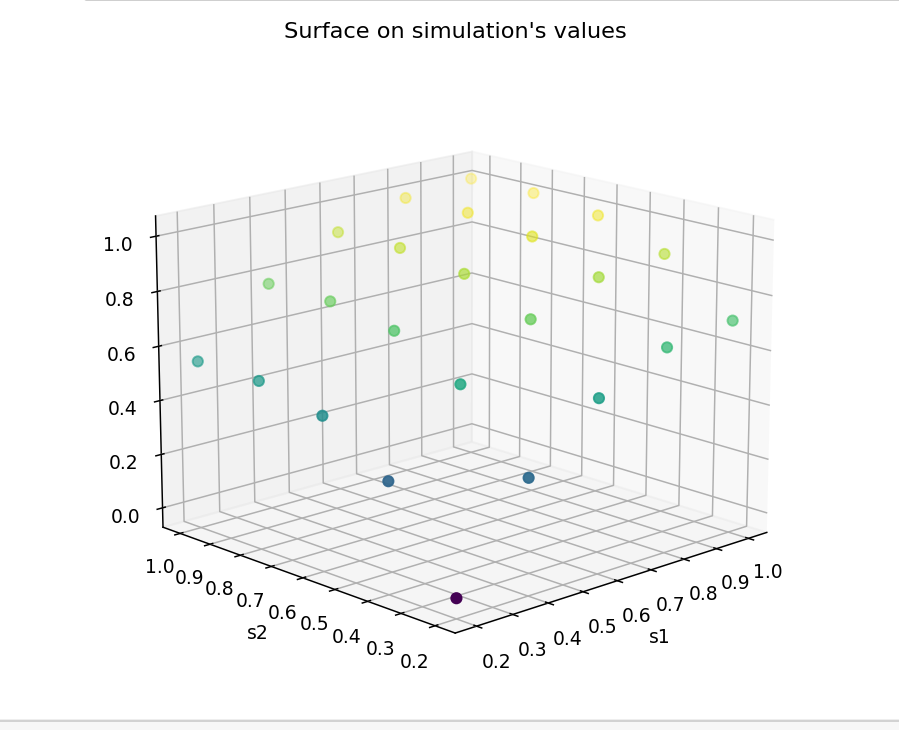
\includegraphics[width=.7\linewidth]{Simulations_values.PNG}
     \caption{Interpolation for Data 1}\label{Fig:Data1}
   \end{minipage}\hfill
   \begin{minipage}{0.48\textwidth}
     \centering
     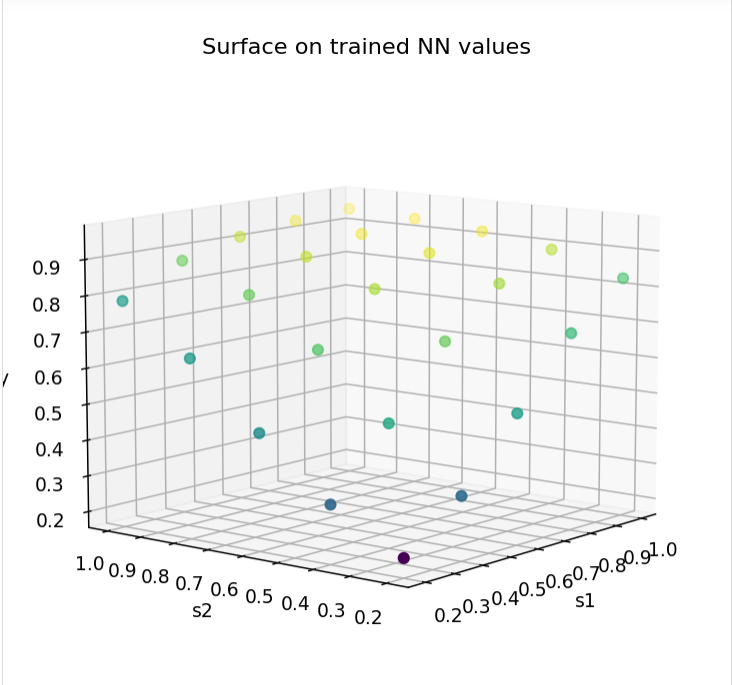
\includegraphics[width=.7\linewidth]{NN_values.PNG}
     \caption{Interpolation for Data 2}\label{Fig:Data2}
   \end{minipage}
\end{figure}



\end{document}

